\pagestyle{fancy}
\chapter*{Heliosismolog\'ia}
\addcontentsline{toc}{chapter}{Heliosismolog\'ia}


Una pregunta importante en el estudio del Sol es ?`C\'omo pueden hacer los f\'isicos solares conocer el interior solar si el mismo no es visible? La forma de hacerlo es justamente la tarea de la Helio-sismolog\'ia que mediante observaciones y medidas de las oscilaciones vistas en la superficie hace inferencias y prospecciones acerca de las propiedades del interior solar. Las medidas que se pueden obtener son medidas en el cambio de la velocidad superficial v\'ia {\it efecto Doppler} a causa del plasma que se mueve hacia adentro y hacia fuera en la l\'inea de la visual del observador, seg\'un el momento en el que se le observe y el {\it modo de oscilaci\'on} predominante bajo el cual est\'e sometido.\\


\section*{Heliosismolog\'ia local}
\addcontentsline{toc}{section}{Heliosismolog\'ia local}

\begin{wrapfigure}[25]{l}{0.5\textwidth}
\begin{center}
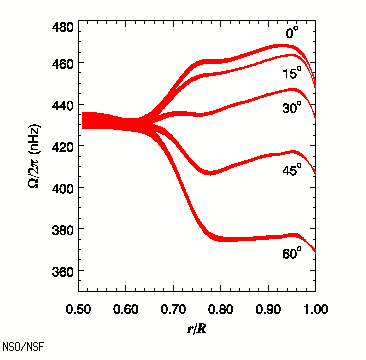
\includegraphics[width=0.5\textwidth]{Tachocline.png}
\caption{Rotaci\'on de la estructura interna solar inferida de los datos heliosismol\'ogicos \citep[]{Thompson1996}.}
\label{fig:rotdiff}
\end{center}
\end{wrapfigure}


% la heliosismologia es una herramienta para estudiar un fen�meno f�sico

%Aparentemente los resultados de Bart sugieren que hay una correlaci�n entre el periodo de las especulas y el periodo fundamental.

% La heliosismologia local fue hecha para tratar de entender la estructura interna de fen�menos locales... por ejemplo una mancha como es una estructura de una mancha por dentro. Como son las cosas por debajo.


%Diagramas de anillo lo �nico que se puede inferiri es la velocidad del sonido... usando un modelo atmosf�rico es que se pueden sacar todos los otros par�metros que se mencionan all�... es un m�todo que se aplica sobre quite sun.


%Cambiar las palabras 3D por tres dimensiones

% Time distance no se limita a los 3mHz

% Duvall gr�fica las croscorrelaciones de las potencias... no es exactamente el diagrama de tiempo.

% revisar articulo de Gizon para lo del time-distance.

%diferenciar: M�todo heliosismol�gico de tiempo distancia. y diagrama tiempo-distancia.

% reescribir la primera parte del subcapitulo 

Dependiendo del tipo de oscilaci\'on en el que se est\'e interesado la {\it heliosismolog\'ia} se divide en {\it global} y {\it local}. Cuando se analizan los modos globales de oscilaci\'on (aquellos que abarcan toda la superficie solar) es posible construir un esquema de la estructura global interna de la estrella. Gracias a esta rama de la f\'isica solar se ha podido lograr establecer, por ejemplo, que la zona de discontinuidad entre la zona radiativa y la zona convectiva conocida como la {\it tacoclina}, aparte de ser una regi\'on en el interior solar donde cambia el mecanismo de transporte de energ\'ia, es tambi\'en un lugar desde el cual el Sol deja de rotar como un cuerpo r\'igido y empieza a hacerlo de forma diferencial y en funci\'on de la latitud heliogr\'afica (ver figura \ref{fig:rotdiff}). Uno de los hallazgos m\'as importantes de esta rama es el llamado {\it modo normal de oscilaci\'on} el cual tiene un periodo cercano a los cinco minutos, una frecuencia asociada de unos $\sim 3$ mHz que ser\'a un valor importante para nosotros en el momento en que toquemos el tema de los mapas de egresi\'on ac\'ustica, y del cual se ha hallado una fuerte correlaci\'on con el periodo de oscilaci\'on de las esp\'iculas \citep[]{DePontieu2004}. Los avances de mayor impacto en esta \'area son expuestos en un art\'iculo de hace una d\'ecada \citep[]{Dalsgaard2002}.\\

La {\it heliosismolog\'ia local} por su lado se centra en el estudio detallado de eventos s\'ismicos mucho m\'as localizados, especialmente sobre aquellos que tienen lugar en regiones activas de la superficie solar. Esto \'ultimo ofrece un nuevo problema a la heliosismolog\'ia y se trata de la forma en la que se desarrolla el tratamiento para dar cuenta de la propagaci\'on de la perturbaci\'on ac\'ustica por debajo de la superficie solar ya que para la determinaci\'on de las propiedades de esa zona hasta entonces se ha apelado exclusivamente a solucionar las ecuaciones hidrodin\'amicas en ausencia de campo magn\'etico, lo cual, por supuesto, deja de ser v\'alido en las regiones activas del Sol que es donde se enfoca el estudio de esta rama. Por otro lado, una ventaja que puede ofrecer el estudio s\'ismico de manchas solares es la posibilidad de desentra\~nar la estructura de estas en el interior solar y a su vez dar visos de la fenomenolog\'ia escondida detr\'as de su aparici\'on y evoluci\'on. Dentro de las prioridades en este momento es encontrar el mejor modelo que de cuenta de la propagaci\'on de una onda ac\'ustica dentro de un plasma acoplado con un campo magn\'etico relativamente fuerte, para enseguida buscar la mejor manera de implementarlo al problema particular de la aparici\'on de un sismo asociado una mancha solar.\\

La Heliosismolog\'ia local es una rama de la f\'isica solar relativamente nueva, desarrollada b\'asicamente durante las \'ultimas dos d\'ecadas desde el reporte por \cite{kz1998}  del primer sismo asociado a una fulguraci\'on tipo X2.6 en la regi\'on activa NOAA 7978. Los datos observacionales para este tipo de an\'alisis han sido tomados por dos instrumentos espaciales y una red de telescopios solares en tierra. Estos son el MDI ({\it Michelson Doppler Imager}) a bordo del SOHO ({\it SOlar and Heliospheric Observatory}) \citep[]{scherrer1995}, el r ecientemente enviado a \'orbita HMI ({\it Helioseismic and Magnetic Imager}) a bordo del SDO ({\it Solar Dynamic Observatory}) \citep[]{kosovichev2007}, y la red de observatorios GONG++ ({\it Global Oscillation Network Group}) \citep[]{harvey1996}. Las im\'agenes que se obtienen son im\'agenes del disco solar completo y la resoluci\'on varia de un instrumento al otro siendo las im\'agenes de MDI y de GONG archivos de $1024\times1024$ p\'ixeles y las de HMI de $4096\times4096$ p\'ixeles, teniendo en cuenta que para los observatorios en tierra se debe considerar adem\'as el efecto producido por la turbulencia atmosf\'erica sobre los datos de ciencia.\\

Para el an\'alisis heliosimol\'ogico local de los Dopplergramas\footnote{Se llaman Dopplergramas a los fotogramas del Sol 2D en los que se marcan diferencias en la velocidad en la componente de la visual.} obtenidos con los instrumentos anteriormente mencionados se han desarrollado una serie de m\'etodos diferentes entre los que se obtiene un acercamiento prospectivo y/o din\'amico. Entre los m\'as utilizados hoy en d\'ia se encuentran el {\it an\'alisis por diagrama de anillos}, los {\it diagramas tiempo-distancia (time distance)} o diagramas TS como se encuentra en alguna literatura, la {\it holograf\'ia ac\'ustica}, la t\'ecnica de {\it Fourier-Hankel}, cada una de ellas utilizada para un fin espec\'ifico que a continuaci\'on discutimos brevemente.


\subsection*{Diagrama de anillos}
\addcontentsline{toc}{subsection}{Diagrama de anillos}

Esta t\'ecnica se basa en cubrir varias regiones peque\~nas en forma de anillos sobre la superficie solar. En cada una de las zonas peque\~nas se infieren dos cantidades f\'isicas que por lo general son la velocidad del sonido y la densidad de masa como funci\'on de la profundidad, y basados en estas, se determinan las otras cantidades como presi\'on y temperatura. Haciendo una combinaci\'on de la informaci\'on de cada zona peque\~na es posible construir una visualizaci\'on en 3D de la estructura interna. Este m\'etodo ha sido usado t\'ipicamente para encontrar el l\'imite externo de la zona convectiva a unos $\sim 30$ Mm de profundidad (siendo esta profundidad usualmente medida desde la alta fotosfera) \citep[]{haber2002}.\\

La forma de proceder es construyendo un espectro de potencia en 3D para cada una de las regiones peque\~nas lo cual resulta en una imagen de anillo \citep[]{hill1988}.\\

Las propiedades del plasma bajo la superficie solar son inferidas mediante el an\'alisis en las variaciones en frecuencias de los espectros de potencia. La presencia de un flujo interno introduce un corrimiento Doppler en las frecuencias, y por lo tanto un cambio en la forma de los anillos. La forma en la que se afectan los diferentes {\it modos} da un indicativo de la profundidad y dimensiones del flujo interno \citep[]{gonzalez2006}. N\'otese que los anillos mostrados en la figura \ref{fig:rotdiff} son construidos a frecuencias muy cercanas a la que hoy d\'ia sabemos que corresponde al modo normal (de resonancia) en el Sol que es el del orden de los cinco minutos \citep[]{goldreich1977} (recordemos que $\nu_{fund}=\frac{1}{T_{fund}}=\frac{1}{300\,s}$=3,3\,\text{mHz}).

\begin{figure}[ht!]
\begin{center}
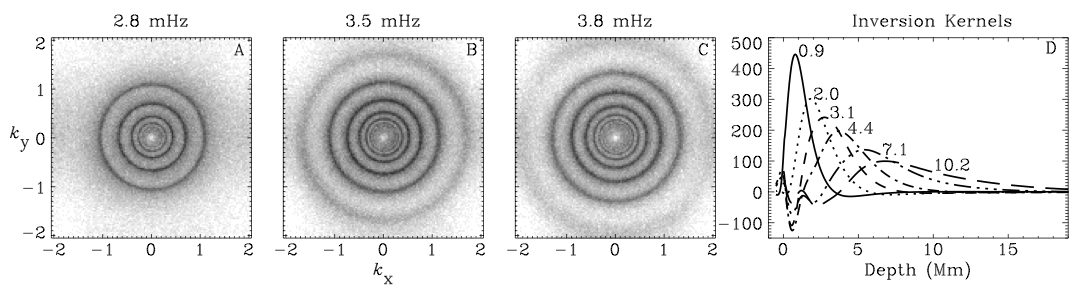
\includegraphics[width=1.0\textwidth]{ringdiagram.png}
\caption{(a) - (c) Corte transversal de un espectro de potencias de un diagrama de anillo tridimensional para tres frecuencias diferentes. Cada anillo corresponde a un \'unico orden radial $n$. (d) N\'ucleos representativos para una inversi\'on basada en los diagramas de anillo graficados como funci\'on de la profundidad bajo la fotosfera \citep[]{haber2002}.}
\label{fig:rotdiff}
\end{center}
\end{figure}

\subsection*{Diagrama de Tiempo-Distancia}
\addcontentsline{toc}{subsection}{Diagrama de Tiempo-Distancia}


Esta t\'ecnica expuesta por primera vez por \cite{duvall1993} se basa en la medida de la trayectoria descrita por una onda ac\'ustica (vista v\'ia efecto Doppler) que viaja de un punto a otro sobre la superficie solar. Esta t\'ecnica es muy usada hoy en d\'ia para la determinar si un cierto evento de fulguraci\'on solar tiene, o no, asociado un sismo. La forma de implementarlo es tomar la imagen Doppler del disco solar obtenida con alguno de los instrumentos dispuestos para esto y recortar la imagen en la zona en donde se produjo la fulguraci\'on para luego centrar sobre ella un c\'irculo cuyo radio va hasta unos 20 Mm y hacer las restas entre im\'agenes consecutivas para encontrar de esta manera la se\~nal de una fuerte variaci\'on ac\'ustica que se propaga desde el centro del c\'irculo hacia afuera de \'el.\\

Este protocolo ya se ha sistematizado y por ejemplo el equipo de la Universidad de Stanford en California encargado del almacenamiento y distribuci\'on de los datos tomados por {\it HMI/SDO} ha construido una serie de programas que cada ocho horas hace un barrido del disco en las fulguraciones que tuvieron lugar durante ese lapso de tiempo y aplican este m\'etodo sobre los Dopplergramas denotados como {\it near-real-time} para determinar la existencia o no de sismos solares \citep[]{zhao2011}. Esto resulta ser una ventaja apreciable ya que se puede informar a la comunidad cient\'ifica mundial la aparici\'on de un nuevo sismo solar en tan solo unas pocas horas despu\'es de que ocurra, tal como ocurri\'o con el primer sismo del ciclo 24 asociado a la fulguraci\'on tipo X2.2 de la regi\'on activa NOAA 1158 que tuvo lugar el 15 de Febrero de 2011 y que tan solo cuatro horas despu\'es fue reportado por Kosovichev \citep[]{kosovichev2011}.\\

\begin{figure}[!ht]
\begin{center}
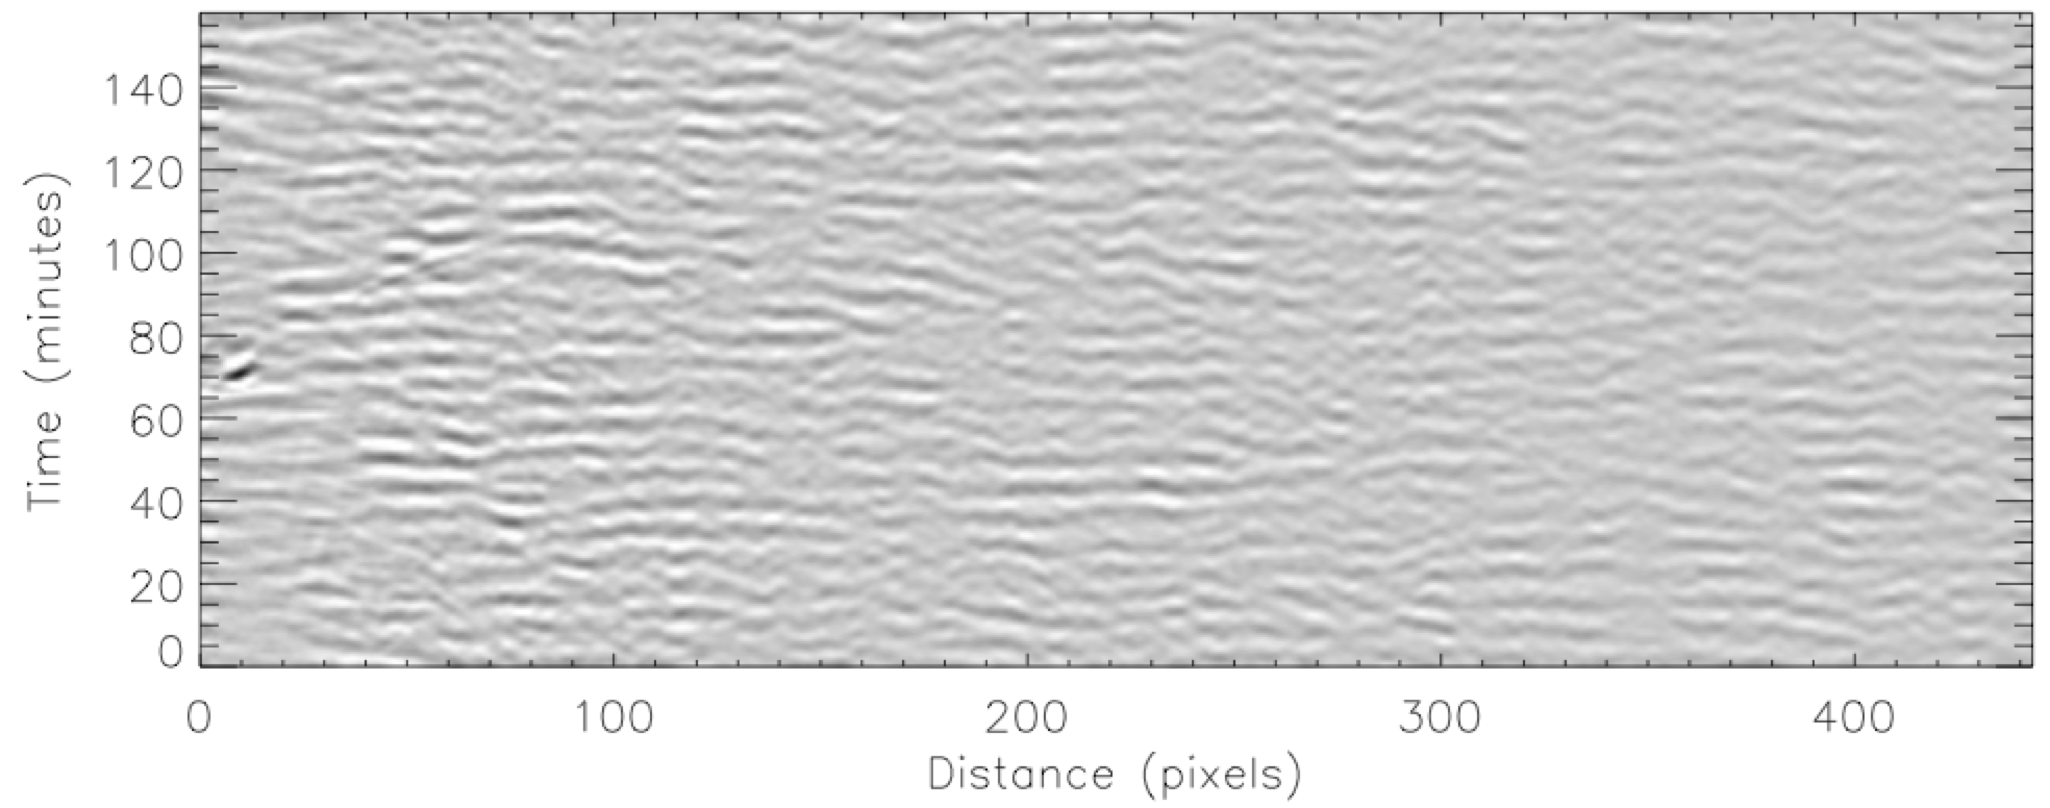
\includegraphics[width=1.0\textwidth]{td_plot_2011_02_15.png}
\caption{Diagrama TD para la fulguraci\'on solar clase GOES X2.2 del 15 de Febrero de 2011. Podemos discernir una se\~nal ac\'ustica ubicada al lado izquierdo que incrementa su velocidad al transcurrir el tiempo.}
\label{fig:td}
\end{center}
\end{figure}

Los principales progresos en la heliosismolog\'ia de la d\'ecada pasada ocurrieron a trav\'es del an\'alisis de los modos normales de oscilaci\'on \citep[]{dalsgaard1991}, esto debido principalmente a la dificultad de observar el viaje temporal de se\~nales ac\'usticas que se confunden con el ruido provocado por los muchos modos de oscilaci\'on que llegan a la superficie solar. Esto entra en contraste con la forma de hacer s\'ismica en nuestro planeta en donde mediante la medida de diferencias de tiempo y diferencias de distancia medidas a trav\'es de diferentes estaciones ubicadas en varios puntos de la superficie terrestre se puede desarrollar una prospecci\'on del subsuelo mediante el an\'alisis espacio temporal de estas se\~nales \citep[]{gubbins1990}.  La t\'ecnica del diagrama Tiempo-Distancia trata de emular esta forma de hacer s\'ismica aqu\'i en la tierra y haciendo uso de los datos de mejor resoluci\'on y observando eventos de fulguraciones solares puede seguir la respuesta sobre la superficie de este tipo de se\~nales como lo reportaron por primera vez \cite{kz1998}.\\

La causa de la perturbaci\'on s\'ismica que da lugar a las ondas vistas despu\'es de un evento de fulguraci\'on solar es un problema abierto de la f\'isica solar que es discutido en los m\'as importantes congresos que se celebran en est\'a \'area y a donde asisten los cient\'ificos m\'as reconocidos y de m\'as amplia trayectoria que trabajan en estos temas \citep[]{zharkova2011a}. Para efectos de entender la forma en la que un frente de 	onda ac\'ustica se propaga por el interior solar para luego ser registrada en una diagrama TD vamos a suponer simplemente que la fuente s\'ismica existe, que es muy fuerte y que est\'a bien localizada.\\

La forma en la que ampliamente se concibe la trayectoria de una onda ac\'ustica cuya fuente est\'a ubicada cerca de la superficie solar es esquematizada en el diagrama de rayos de la figura \ref{fig:td}. Una fuente que tiene lugar en el punto $a$ de la superficie solar es el punto de partida de un rayo que es refractado debido al incremento de la velocidad del sonido local del medio en el que se propaga hasta invertir su direcci\'on radial y llegar al punto $c$. Una vez llega a $c$ se encuentra con un cambio brusco en la densidad local, raz\'on por la cual la onda es reflejada y contin\'ua una trayectoria similar hacia otro punto sobre la superficie solar. De esta manera es como se presenta una correlaci\'on entre el frente de onda visto en $c$ y el punto $a$ desde el cual se origin\'o. La distancia que se observa es la que est\'a sobre la superficie $\Delta$ pero claramente el camino recorrido es $b$ a trav\'es del interior solar. Si la fuente ac\'ustica tuvo lugar en el tiempo $t$, entonces decimos que el tiempo caracter\'istico que tarda el frente de onda de ir desde el punto $a$ hasta el punto $c$ es $T$ y al que se le conoce como el {\it tiempo de viaje}. A pesar de esta relaci\'on directa entre los dos puntos sobre la superficie solar $a$ y $c$, las se\~nales que se observan se ven afectadas por un ruido apreciable introducido por todas aquellas perturbaciones {\it extras} que presentan de forma aleatoria a lo largo del camino $b$ y que a pesar de ser de menor intensidad, tambi\'en tienen una respuesta que es vista en los mismos dos puntos $a$ y $c$. La literatura se refiere a esta interferencia como el {\it problema de oblicuidad}. Es por esta misma raz\'on que no se puede construir un espectro de potencia unidimensional en una l\'inea de p\'ixeles definida sobre una imagen solar, sino que en vez de esto se debe realizar un an\'alisis que abarque una circunferencia centrada en la fuente del sismo.\\

\begin{wrapfigure}[22]{l}{0.45\textwidth}
\begin{center}
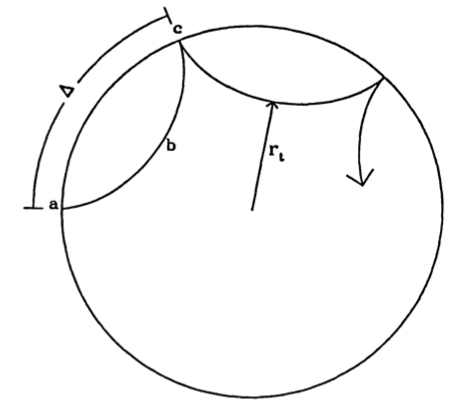
\includegraphics[width=0.42\textwidth]{td.png}
\caption{Esquema que muestra el camino por el que se propaga una onda sonora a lo largo del interior solar. Tomado de \citep[]{duvall1995}}
\label{fig:td}
\end{center}
\end{wrapfigure}

Los primeros trabajos en los que se implement\'o este m\'etodo TD se encontraron {\it tiempos de viaje} del orden de los 75 minutos y distancias $\Delta$ del orden de 25 grados de arco heliosf\'ericos \citep[]{duvall1995} mucho mayor a los tiempos y distancias reportados en los sismos asociados a eventos de fulguraci\'on solar en las vecindades de las manchas solares (ver por ejemplo \citep[]{kosovichev2011,martinez-oliveros2009,mo2008d,metal2006b,detal2006}) en los que los tiempos de viaje son del orden de los 30 minutos y las distancias son cercanas a los 5 o 10 grados heliosf\'ericos. La raz\'on es que a pesar de que el diagrama TD es un m\'etodo centrado en una localidad finita de la superficie solar, en un principio fue usado dentro del marco de la heliosismolog\'ia global bajo la suposici\'on de un n\'umero de {\it Reynolds magn\'etico} grande de manera que son los {\it modos-p} la base sobre la cual el frente de onda ac\'ustico se propaga. Claramente, el plasma confinado en una mancha solar se comporta siguiendo un r\'egimen magn\'etico de manera que las l\'ineas de campo magn\'etico se encuentran congeladas y los modos-p de vibraci\'on son amortiguados fuertemente \citep[]{braun1988,dsilva1995}.\\

Los diagramas de tiempo-distancia trabajados por \cite{duvall1995} est\'an centrados principalmente en un sector de {\it Sol calmo} pero la perturbaci\'on ac\'ustica que se propaga con el tiempo logra entrar luego en una regi\'on activa en donde se visualiza una fractura de la trayectoria y despu\'es de un corto tiempo se observa una disminuci\'on en la intensidad de la se\~nal y una descomposici\'on en su banda de l\'ineas que, se cree, es debido a la presencia de campo magn\'etico dentro de la mancha a trav\'es de la cual contin\'ua propag\'andose la perturbaci\'on. Esto sugiere que la forma en la que se da esta fractura y la posterior aparici\'on de una banda de curvas puede estar relacionada fuertemente con la estructura interna de la mancha solar y es esta la principal raz\'on por la que hoy d\'ia es un tema que genera un gran apetito cient\'ifico para los f\'isicos solares, pues un estudio detallado de este fen\'omeno podr\'ia ayudar a construir un mayor entendimiento de la estructura sub-superficial del Sol.\\

Para explicar la disminuci\'on de la intensidad de la se\~nal ac\'ustica, una vez la perturbaci\'on entra a la mancha solar, se apela a pensar en fen\'omenos de difusi\'on ac\'ustica que aten\'uen la onda. Para dar cuenta de esto desde un acercamiento netamente fenomenol\'ogico se hacen algunas hip\'otesis como que a trav\'es de la mancha solar, y de forma completamente perpendicular, atraviesa un tubo magn\'etico monol\'itico que incrementa la disipaci\'on de los modos ac\'usticos al pasar por las capas resonantes y el un conglomerado de fibrillas internas del tubo adem\'as de la atenuaci\'on debida a la conversi\'on de modos {\it ac\'usticos} a modos {\it magneto-ac\'usticos}. Una revisi\'on detallada de la matem\'atica propuesta para describir esta din\'amica se encuentra en \cite{spruid1992,dsilva1995,dsilva1996,dsilva2001} y \cite{kosovichev2011td}.\\

Una de las debilidades m\'as remarcadas de este m\'etodo es aquella que concierne al ruido que se filtra en los diagramas TD como bien se puede ver, por ejemplo, de aquel que construimos para el evento del 15 de Febrero de 2011 (ver figura \ref{fig:td}) y m\'as a\'un la {\bf raz\'on se\~nal-ruido} de la supuesta propagaci\'on ac\'ustica que se registra. En aras de dar soluci\'on a este problema se ha tratado de caracterizar el ruido ac\'ustico considerando a los mecanismos de excitaci\'on de los modos como fen\'omenos de naturaleza estoc\'astica que generan oscilaciones estacionarias y homog\'eneas sobre toda la superficie solar. De esta manera es posible construir una matriz de covarianza entre las medidas del tiempo de viaje y la inversi\'on ac\'ustica que resulta de este tipo de an\'alisis:

\begin{align}
C(\mathbf{x}_1,\mathbf{x}_2,t_j)=\frac{h_t}{T-|t_j|}\sum_i\phi(\mathbf{x}_1,t_i)\phi(\mathbf{x}_2,t_i+t_j),
\end{align}

\noindent donde $\phi(\mathbf{x},t)$ denota la se\~nal ac\'ustica filtrada observada para un punto $\mathbf{x}$ en un instante\footnote{Este filtrado se realiza mediante la aplicaci\'on de un par de operadores en el dominio del espacio de Fourier del conglomerado de datos observados que generalmente es la remoci\'on de todas aquellas oscilaciones que son m\'ultiplos enteros del modo fundamental de oscilaci\'on y un filtro Gaussiano en fase con la velocidad de la forma $\exp[-(\omega/k-v)^2/(2s^2)]$ siendo $v=36.5\,\text{km s}^{-1}$ y $s=2.5\,\text{km s}^{-1}$.} $t$, $h_t$ es la cadencia del instrumento con el que son tomadas las im\'agenes, $t_j=jh_t$ con $j\,\epsilon\, Z$, y $T$ es el tiempo total sobre el cual se est\'a haciendo el an\'alisis. Un trabajo completo en el que se desarrolla este m\'etodo de limpieza del ruido en la se\~nal y se compara con datos observacionales reales obtenidos con MDI/SOHO es mostrado en \cite{gizon2004}. Como vemos el proceso de filtrado de la se\~nal ac\'ustica genera una repercusi\'on apreciable sobre las medidas de manera que se debe tener en cuenta a la hora de intentar hacer alguna interpretaci\'on f\'isica de las observaciones, como bien lo indican \cite{braun2008,chou2009,salabert2009} y \cite{donea2011}. Este es un m\'etodo que se ha convertido en una herramienta potente de la f\'isica solar, pero que a\'un hoy en d\'ia se discuten sus problemas, como fue el caso del \'ultimo encuentro {\it AGU-2010} ({\it American Geophysical Union}) en donde \cite{duvall2010} expuso el estado del arte de este tema.

\section*{Holograf\'ia heliosismol\'ogica}
\addcontentsline{toc}{section}{Holograf\'ia heliosismol\'ogica}

El m\'etodo de {\it holograf\'ia heliosismol\'ogica} es una t\'ecnica cuya finalidad es la reconstrucci\'on tridimensional de la morfolog\'ia interna de la atm\'osfera solar basandose en la propagaci\'on de los modos-p y la forma en que estos se registran en la superficie del Sol. En Octubre de 1997 Chang y sus colaboradores proponen el m\'etodo llamado {\it imaginolog\'ia ac\'ustica} que consiste en la observaci\'on del ruido ac\'ustico sobre la superficie solar suponiendo que ha sido generado de forma homog\'enea en su interior de manera que (asumiendo adem\'as un primer modelo de la estructura interna de la capa m\'as externa del Sol, la {\it atm\'osfera solar}) si no hubiese ning\'un tipo de obst\'aculo las se\~nales alcanzar\'ian la superficie con cierta fase. El no encontrar las se\~nales ac\'usticas con la fase esperada supondr\'ia la existencia de un obst\'aculo ``{\it \'optico}'' interno y la forma de dimensionarlo ser\'ia justamente aplicando un m\'etodo an\'alogo al usado en \'optica cl\'asica cuando con ayuda de un montaje \'optico se registra la se\~nal de una fuente de luz en cuyo camino \'optico se ha atravesado un obst\'aculo que dispersa los rayos. Esta t\'ecnica fue inicialmente pensada para poder generar la imagen de prospecci\'on interna de inhomogeneidades en el plasma solar tales como las que se presentan en el surgimiento de manchas solares \citep[]{chang1997}. Para ese mismo a\~no los doctores Charles Lindsey y Douglas Braun publican un art\'iculo en el que por primera vez proponen la {\bf holograf\'ia heliosismol\'ogica} como un m\'etodo de prospecci\'on ac\'ustica que permite la ubicaci\'on de la fuente de sismos fuertemente localizados en la superficie del Sol \citep[]{lindsey1997}.\\


\begin{wrapfigure}[28]{l}{0.45\textwidth}
\begin{center}
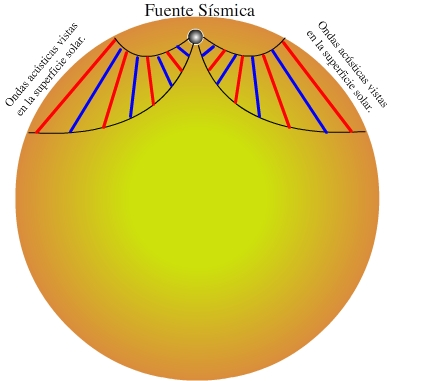
\includegraphics[width=0.42\textwidth]{helioholography.jpg}
\caption{Figura que representa la propagaci\'on de una se\~nal ac\'ustica en el interior solar cerca de la superficie. El dibujo se ha exagerado un poco para hacer \'enfasis en la retro-dispersi\'on que se presenta producto del incremento gradual de la densidad de masa con la profundidad, as\'i como tambi\'en del \'indice {\it \'optico} del medio. Las l\'ineas azules y rojas representan picos y valles de la se\~nal. Se asume un medio cuyas propiedades f\'isicas cambian \'unicamente con la direcci\'on radial.}
\label{fig:holografia}
\end{center}
\end{wrapfigure}


Mucho del tratamiento matem\'atico que se usa en la {\bf holograf\'ia ac\'ustica} es an\'alogo y tomado del formalismo definido sobre la holograf\'ia \'optica propuesta por el cient\'ifico H\'ungaro-Brit\'anico {\it Dennis Gabor} en 1947 y por el cual gan\'o el premio nobel de f\'isica en 1971 \citep[]{collier1971}. En este contexto, el registro de un patr\'on dos-dimensional generado por una superposici\'on de ondas sonoras se considera un {\bf holograma ac\'ustico}. Entonces, haciendo uso de estos {\it hologramas} es posible realizar una prospecci\'on del campo de ondas ac\'usticas que han viajado a trav\'es de un espacio tridimensional del cual se conocen sus caracter\'isticas generales como composici\'on y topolog\'ia\footnote{La {\it topolog\'ia} del medio por el cual se propagan las ondas ac\'usticas cobra una importancia sobresaliente cuando la propagaci\'on se hace sobre un medio que no es isotr\'opico y/o homog\'eneo,  ya que la din\'amica de propagaci\'on de las ondas cambia completamente y empieza a depender por ejemplo de la direcci\'on en la que se propague un frente de onda.}.\\

\noindent El caso m\'as sencillo de suponer es un medio de propagaci\'on uniforme y homog\'eneo dentro del cual se encuentra una fuente de ondas ac\'usticas que se propagan y son registradas en alg\'un lugar durante un periodo de tiempo determinado\footnote{Obviamente la atm\'osfera solar no es un medio uniforme y homog\'eneo a trav\'es del cual se propagan las ondas; por esta raz\'on, para poder hacer holograf\'ia ac\'ustica es ineludible ajustarse a un modelo de atm\'osfera estelar.}. En general, un holograma es generado cuando sobre una superficie ``{\it plana}'' se graba la superposici\'on de la llegada de dos o m\'as ondas provenientes de iluminar el objeto de estudio desde diferentes lugares (diferentes {\it perspectivas}). Para poder obtener un holograma ac\'ustico asociado a un evento de sismo localizado en la superficie solar se hacen un par de suposiciones moderadas para crear un primer acercamiento a esta construcci\'on. Primero se supone una atm\'osfera solar cuyas propiedades f\'isicas no cambian con la latitud y la longitud heliogr\'aficas; esto es, se dice que por ejemplo la densidad cambia solo con la profundidad de la atm\'osfera solar, siguiendo por ejemplo un modelo como el propuesto por \cite{benz2002} (ver figura \ref{corona-heating}). Adem\'as, se plantea una fuente s\'ismica muy bien localizada ({\it casi-puntual}) en el interior solar, de manera que hay una cierta simetr\'ia en las ondas cuando salen de all\'i. Para analizar la forma en la que aplica esta t\'ecnica sobre la superficie solar, consideremos la situaci\'on planteada en la figura \ref{fig:holografia}. All\'i se presenta una fuente de ondas ac\'usticas cerca de la superficie solar. La parte de la se\~nal sonora que va hacia adentro del Sol sufre una retro-dispersi\'on a causa del aumento de la densidad de masa, a lo cual se asocia tambi\'en un aumento gradual en el valor del \'indice ``{\it \'optico}'' del medio de propagaci\'on\footnote{La manera en la que la fuente de la se\~nal ac\'ustica es generada es un tema de fuerte debate a\'un hoy en d\'ia y su discusi\'on se present\'o en el subcap\'itulo de {\bf sismicidad asociada a fulguraciones solares}.}.\\

El formalismo te\'orico detr\'as de la holograf\'ia ac\'ustica es relativamente simple y completamente an\'alogo al usado en holograf\'ia \'optica. Un frente de onda definido sobre una longitud de onda part\'icular se puede representar mediante un n\'umero complejo $\mathbf{U}$, en donde la amplitud y la fase del frente de onda son el valor absoluto y el \'angulo del n\'umero complejo respectivamente. Si sobre la ``{\it pantalla}'' en la que se construye el holograma est\'an incidiendo dos frentes de onda provenientes de dos lugares distintos desde los cuales se ilumina el objeto, cada uno de estos frentes de onda puede ser representado por un n\'umero complejo que llamamos $\mathbf{U}_1$ y $\mathbf{U}_2$, de manera que la combinaci\'on de estos dos se reduce a su suma, $\mathbf{U}_1+\mathbf{U}_2$. La energ\'ia de esta superposici\'on de rayos est\'a dada por

\begin{align}\label{u1+u2}
|\mathbf{U}_1+\mathbf{U}_2|^2=|\mathbf{U}_1|^2+|\mathbf{U_2}|^2+\mathbf{U}_1\mathbf{U}_2^*+\mathbf{U}_1^*\mathbf{U}_2
\end{align}

\noindent en donde los dos primeros t\'erminos de la derecha son las intensidades de las ondas $\mathbf{U}_1$ y $\mathbf{U}_2$, mientras que los dos \'ultimos t\'erminos representan las intensidades adicionales debido a la interferencia entre los dos frentes de onda. Cuando el rayo del objeto y el rayo de referencia provienen de direcciones apreciablemente diferentes, los frentes de onda de la imagen virtual, real y de referencia emergen con diferentes \'angulos siendo posible reconstruir el objeto y verlo claramente.\\

\begin{wrapfigure}[16]{r}{0.53\textwidth}
\begin{center}
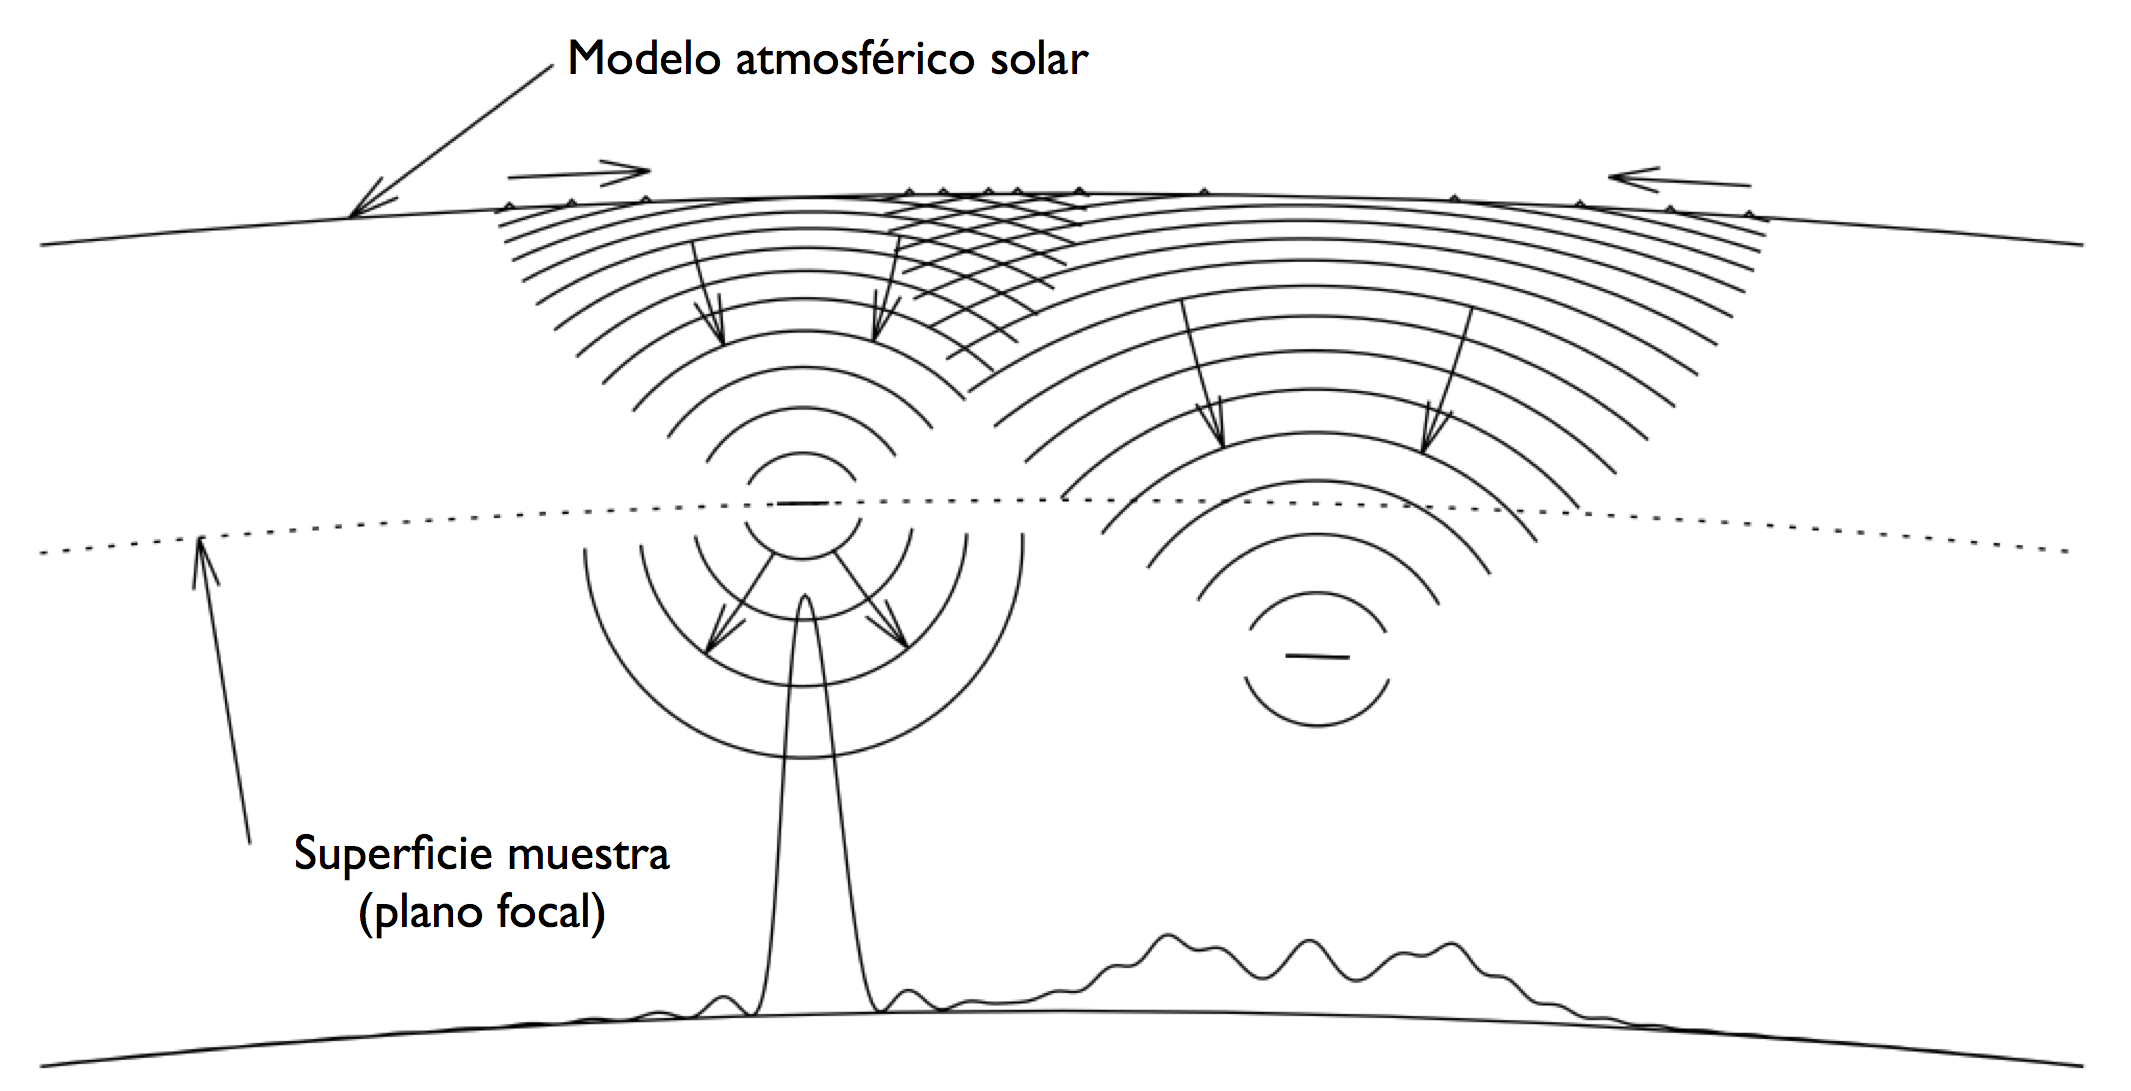
\includegraphics[width=0.51\textwidth]{acustico.png}
\caption{Representaci\'on de una regresi\'on hologr\'afica basada en un campo ac\'ustico observado en la superficie solar. Figura tomada de \cite{lb2000}.}
\label{fig:acustico}
\end{center}
\end{wrapfigure}

La holograf\'ia heliosismol\'ogica (en t\'erminos muy generales) toma las oscilaciones observadas en la superficie solar y calcula la ``imagen s\'ismica'' a cierta profundidad del Sol. Cuando esta es calculada hacia adelante en el tiempo se le llama imagen, o mapa, de {\bf egresi\'on}, mientras que cuando se calcula hacia atr\'as en el tiempo se le llama imagen, o mapa, de {
\bf ingresi\'on}. El ejercicio de diagn\'ostico b\'asico de la holograf\'ia s\'ismica consiste en aplicar una inversi\'on temporal sobre un conjunto de observaciones s\'ismicas de la superficie solar bas\'andose en un modelo computacional de la atm\'osfera solar desprovisto de fuentes, sumideros o dispersiones ac\'usticas. En general, esta t\'ecnica debe aplicarse sobre una regi\'on limitada de la superficie solar. Abusando del lenguaje propio de la \'optica a la regi\'on sobre la que se aplica este procedimiento se le llama la {\it pupila}. Una vez se define esta pupila sobre los par\'ametros de entrada del c\'odigo num\'erico y este se corre, las ahora entrantes perturbaciones ac\'usticas convergen todas juntas al punto donde se localiz\'o la fuente ac\'ustica. Si se toma una muestra de la potencia ac\'ustica en una superficie, i.e., en un ``{\it plano focal}'', a la profundidad en la que tuvo lugar la fuente ac\'ustica, el resultado ser\'a una se\~nal intensa y bien definida cuyo ancho estar\'a definido por el l\'imite de difracci\'on de la se\~nal, tal y como aparece debajo de la fuente en la parte izquierda de la figura \ref{fig:acustico}. De otro lado, si el plano focal es movido hacia arriba o hacia abajo de la profundidad a la cual se present\'o la fuente, la se\~nal en general no desaparece pero s\'i se desenfoca apreciablemente, observ\'andose un perfil difuso como el que se esquematiza en la parte baja del lado derecho de la figura \ref{fig:acustico}.\\

Considerando un medio continuo, libre de fuentes, sumideros y/o puntos de dispersi\'on, a trav\'es del cual se propaga un tren de ondas, bastar\'ia conocer la amplitud y la derivada de esta en un tiempo dado para poder extrapolar el campo ac\'ustico a trav\'es de todo el interior solar y todo tiempo por medio de la soluci\'on de la integral de Kirchhoff \citep[]{born1975}. Este tipo de procedimientos suponen una distribuci\'on {\it continua} de datos, que por obvias razones no se puede obtener de las observaciones heliosismol\'ogicas, raz\'on por la cual a pesar de que esta soluci\'on (la de la integral de Kirchhoff) pueda representar una componente significativa del campo ac\'ustico subyacente, {\bf no} debe ser considerada como una soluci\'on que de cuenta del campo ac\'ustico {\it real} ya que el medio a trav\'es del cual se propagan las ondas est\'a permeado de un mont\'on de anomal\'ias f\'isicas. De esta manera es que se encuentra la necesidad de establecer la diferencia entre el campo ac\'ustico obtenido mediante la aplicaci\'on de un modelo te\'orico de egresi\'on, $H$, y el campo ac\'ustico {\it real}, $\psi$. \cite{lindsey1997} establecen que estos dos \'ultimos campos se relacionan mediante una funci\'on de {\it Green} que da cuenta de la propagaci\'on hacia adelante y hacia atr\'as en el tiempo, $H_+(\mathbf{r},z,t)$ y $H_-(\mathbf{r},z,t)$ respectivamente.  A $H_+(\mathbf{r},z,t)$ se le suele llamar la ``{\it egresi\'on ac\'ustica}''que se relaciona con $\phi$ mediante la siguiente expresi\'on

\begin{align}\label{egresion}
H_+(\mathbf{r},z,t)=\int \, dt'\int_{a<|\mathbf{r}-\mathbf{r}'|<b}\,d^2\mathbf{r}'G_+(|\mathbf{r}-\mathbf{r}'|,z,t-t')\phi(\mathbf{r}',t'),
\end{align}

\begin{wrapfigure}[22]{r}{0.58\textwidth}
\begin{center}
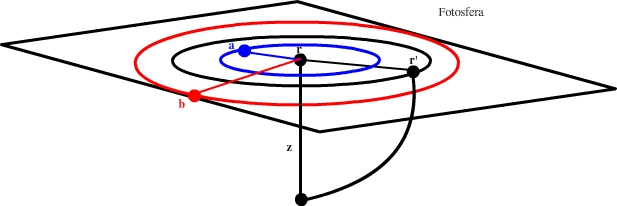
\includegraphics[width=0.56\textwidth]{egresion.jpg}
\caption{Figura que esquematiza la pupila usada en la t\'ecnica de holograf\'ia ac\'ustica sobre la superficie del Sol, en donde se resalta que se usa una pupila anular con radio interior $a$ (azul) y radio exterior b (rojo). Adem\'as que el mapa de egresi\'on es calculado sobre el punto $\mathbf{r}$ cuando las perturbaciones son vistas a lo largo de la circunferencia de radio $\mathbf{r}'$. Seg\'un esta t\'ecnica la fuente ac\'ustica se encuentra a una profundidad $z$ y la trayectoria del frente de onda es una curva debido al cambio de densidad del medio por el cual ella se propaga.}
\label{fig:egresion}
\end{center}
\end{wrapfigure}

\noindent en donde $G_+$ es la funci\'on de {\it Green} que expresa c\'omo una perturbaci\'on registrada en un punto transitorio \'unico en $(\mathbf{r},z,t)$, en el interior solar, se propaga hacia las capas m\'as externas hasta alcanzar la superficie en donde se registra el frente de onda viajero en $(\mathbf{r}',0,t')$. Por otra lado, la {\it ingresi\'on ac\'ustica}, $H_-$, es la inversi\'on temporal de la {\it egresi\'on ac\'ustica} $H_+$. Esta {\it ingresi\'on} da cuenta de las ondas que de manera coherente convergen todas juntas a un mismo punto focal en $(\mathbf{r},z)$. La {\it ingresi\'on} puede ser calculada si en la ecuaci\'on \ref{egresion} se usa como factor integrante la funci\'on de {\it Green} 

$$
G_-(|\mathbf{r}-\mathbf{r}'|,z,t-t').
$$

\noindent Esta funci\'on de {\it Green}, m\'as conocida como la funci\'on {\bf iconal} de {\it Green}, que solo depende de la direcci\'on radial gracias a la suposici\'on de simetr\'ia acimutal que se presenta en la superficie solar (cuando se habla de su estructura), puede ser descrita como un producto entre una funci\'on delta y una funci\'on $f$ que da cuenta del decremento de la amplitud de la perturbaci\'on a medida que se propaga:

\begin{align}
G_+(|\mathbf{r}-\mathbf{r}'|,z,t-t')=\delta[(t-t')-T(|\mathbf{r}-\mathbf{r}'|,z)]f(|\mathbf{r}-\mathbf{r}'|,z),
\end{align}

\noindent donde $T$ es el tiempo transcurrido entre la generaci\'on del pulso y la llegada del frente de onda al punto $\mathbf{r}'$ sobre la superficie visible del Sol. Esta representaci\'on caracteriza la din\'amica ac\'ustica del modelo solar en el que se construye una regresi\'on ac\'ustica mediante el uso de las observaciones helios\'ismicas. La holograf\'ia s\'ismica computacional ha sido desarrollada como una t\'ecnica de diagn\'ostico muy flexible de manera tal que {\bf no} est\'e restringida a un modelo de atm\'osfera solar particular. En este sentido, la funci\'on de {\it Green} puede alejarse considerablemente de lo que ser\'ia el interior solar ac\'ustico real y sin embargo seguir proporcionando im\'agenes de muy alta calidad y \'utiles para diagnosticar la ubicaci\'on de la fuente s\'ismica.\\


En aras de calcular la potencia ac\'ustica de egresi\'on \citet{lb2000} proponen hacer el c\'alculo de la ecuaci\'on (\ref{egresion}) en el dominio de las frecuencias y el n\'umero de onda; \'esto con el fin de eliminar las integraciones en el anillo y trabajar m\'as bien en forma operacional:

\begin{align}
\hat{H}_+(\mathbf{k},z,\nu)=\hat{G}_+(|\mathbf{k}|,z,\nu)\hat{\psi}(\mathbf{k},\nu),
\end{align}

\noindent donde $\hat{H}_+$, $\hat{G}_+$ y $\hat{\psi}$ son las {\it transformaciones de Fourier} en espacio y tiempo de $H_+$, $G_+$ y $\psi$, respectivamente. En este cambio se trabaja con los modos normales de oscilaci\'on ac\'ustica cuyas proyecciones sobre la superficie solar  (en la aproximaci\'on de un plano horizontal) resultan ser simplemente ondas planas viajeras. De aqu\'i la importancia de que en esta t\'ecnica, antes de entrar a aplicar la holograf\'ia ac\'ustica sobre los datos crudos reales, sea necesario realizar una proyecci\'on del disco solar que preserve las distancias verdaderas entre dos puntos contenidos en la superficie solar. Una descripci\'on detallada de esta t\'ecnica se encuentra en \cite{lindsey1997,lb2000}.

\subsection*{Proyecci\'on Postel}
\addcontentsline{toc}{subsection}{Proyecci\'on Postel}


Como vimos en la secci\'on anterior, particularmente cuando nos referimos a la figura \ref{fig:egresion}, se tiene un centro y diferentes se\~nales que arriban a la superficie desde profundidades diversas. Ahora bien, esto lo observamos en un plano de imagen; sin embargo, al Sol lo podemos suponer esf\'erico, y por lo tanto, necesitamos hacer una proyecci\'on de la descripci\'on de las se\~nales estudiadas  en un plano de imagen, si bien provienen de una superficie (solar) curva. A este tipo de proyecci\'on se le conoce en la literatura como {\it proyecci\'on azimutal equidistante} o {\it proyecci\'on Postel} por aquello de que fue usada por {\it Guillaume Postel} en la contrucci\'on de algunos mapas geogr\'aficos en 1581 \citep[]{snyder1926}. Este procedimiento consiste en generar la proyecci\'on de diversos puntos ubicados sobre la superficie esf\'erica, en un plano tangente a la esfera en el punto {\bf P}, como  se muestra en la figura \ref{fig:postel}, de manera que con respecto a este punto {\bf P} se preservan tanto las distancias como los \'angulos entre los puntos ubicados a lo largo de circunferencias conc\'entricas\footnote{Este tipo de proyecci\'on es el que se usa en el globo terrestre que se ha establecido como emblema de la {\it Organizaci\'on de las Naciones Unidas}.} en {\bf P}. 

% Comentario: Averiguar si la proyecci�n Postel es una proyecci�n CONFORME: S� lo es


La construcci\'on de la proyecci\'on Postel se lleva a cabo fijando un punto sobre la superficie solar de coordenas heliogr\'aficas $\theta$, $\varphi$ de manera que las coordinas sobre el mapa plano de todos los otros puntos se hallan mediante 

\begin{align}\label{eq:postel}
\left\{
\begin{array}{c l}      
    X'_p & =\theta'\cos\varphi'\\
    Y'_p & =\theta'\sin\varphi'
\end{array}\right.,
\end{align}

\noindent en donde $\theta'$, $\varphi'$ son unas coordenadas esf\'ericas tales que deben satisfacer que $P$ est\'e en uno de los polos y que se relaciones con $\theta$, $\varphi$ mediante el siguiente conjunto de ecuaciones:

\begin{align}\label{eq:transform}
\left\{
\begin{array}{cl}
\cos\theta'\sin\varphi'&=\cos\theta\sin(\varphi-\varphi_0)\\
\sin\theta'&=-\cos\theta\sin\theta_0\cos(\varphi-\varphi_0)+\sin\theta\cos\theta_0\\
\cos\theta'\cos\varphi'&=\cos\theta_0\cos\theta\cos(\varphi-\varphi_0)+\sin\theta_0\sin\theta
\end{array}\right.,
\end{align}

\noindent siendo $\theta_0$ y $\varphi_0$ las coordenadas del punto $P$ en las antiguas coordenadas esf\'ericas \citep[]{pearson1977}.


\begin{figure}[ht!]
\centering
\subfloat[]{
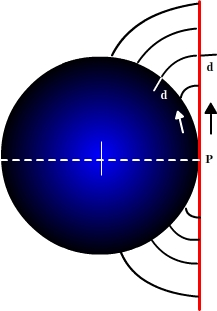
\includegraphics[width=0.2\textwidth]{postela.jpg}}
\subfloat[]{
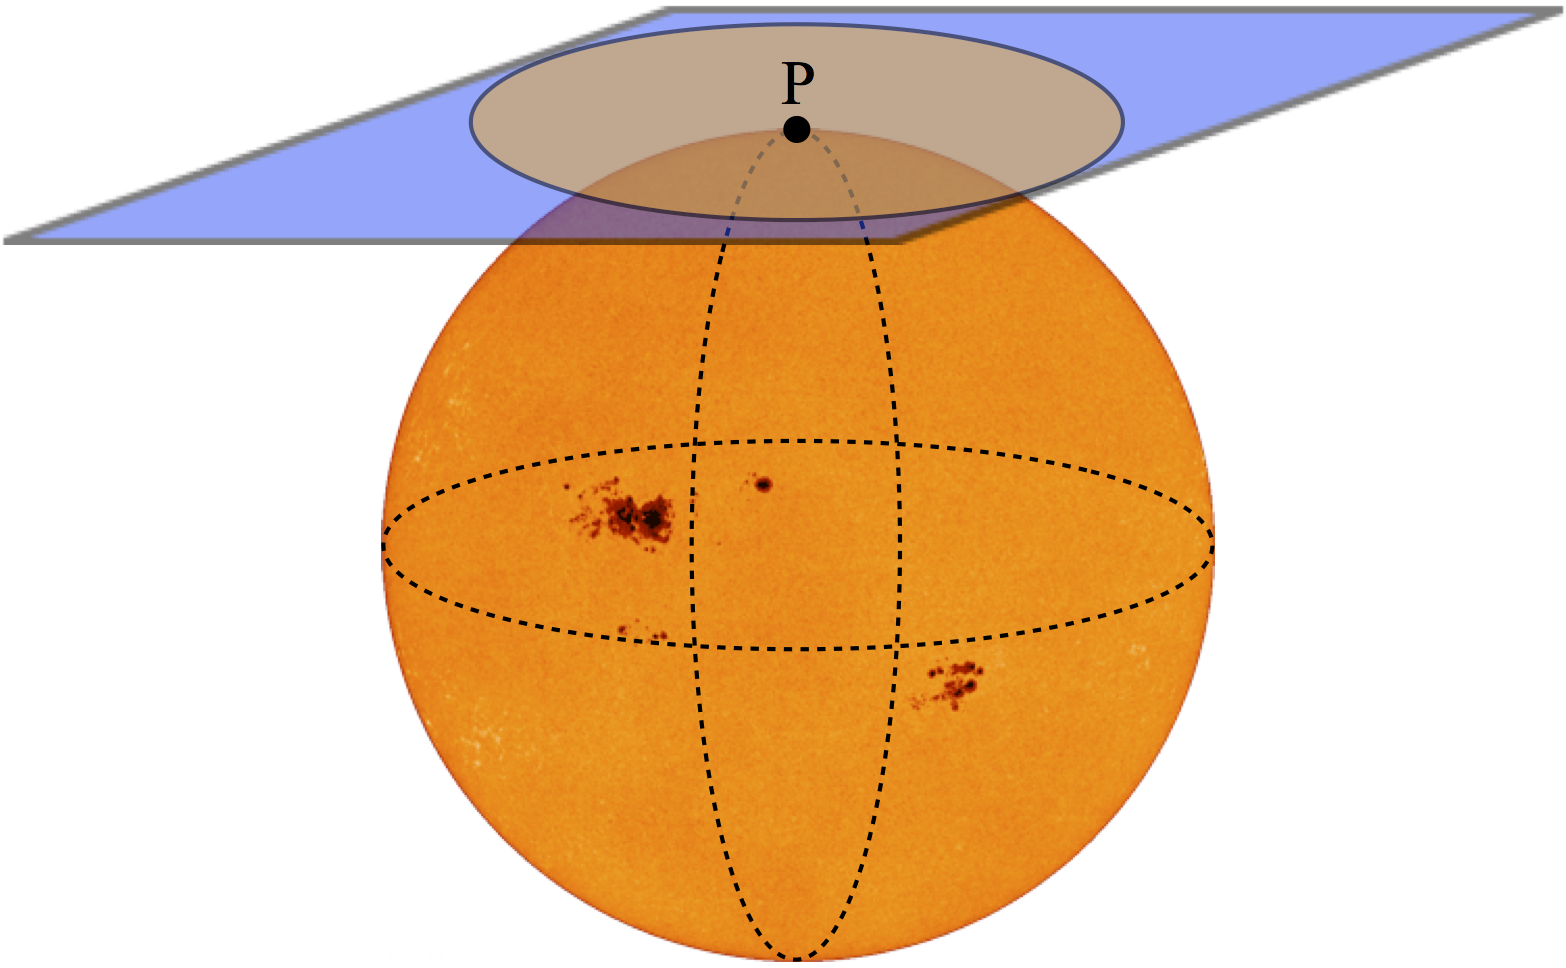
\includegraphics[width=0.37\textwidth]{postelb.png}}
\subfloat[]{
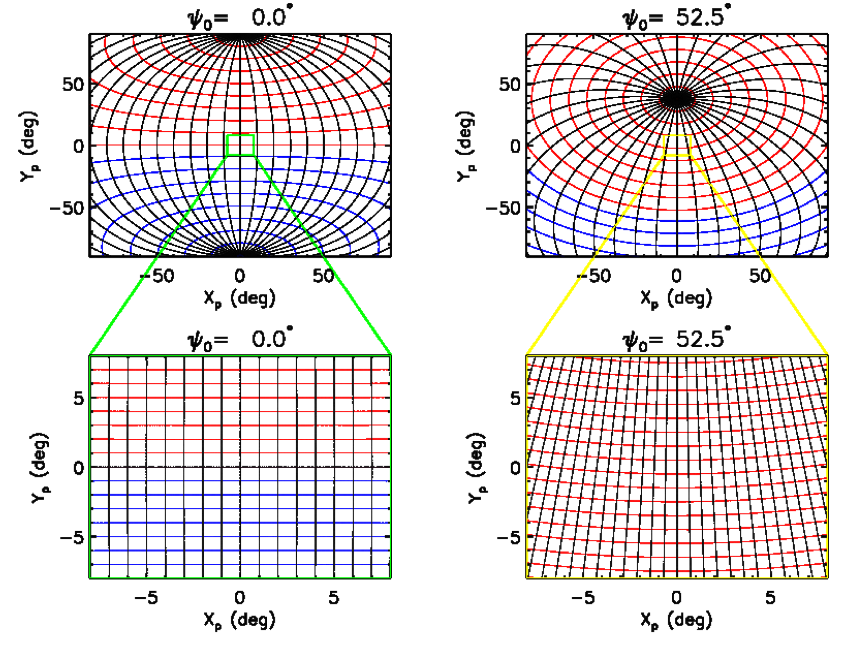
\includegraphics[width=0.37\textwidth]{postelc.png}}
\caption{Conjunto de figuras que esquematizan la proyecci\'on {\it Postel}. (a) Vista en perspectiva de una superficie completamente esf\'erica (azul) que se proyecta sobre un plano (rojo). En este los trazos en negro representan la proyecci\'on de cada uno de los puntos de la esfera sobre el plano y se observa claramente c\'omo las distancias se conservan a lo largo de una l\'inea trazada en direcci\'on radial con centro en el punto P. (b) La proyecci\'on {\it Postel} de la superficie solar centrada en un punto P ubicado en uno de los polos helioc\'entricos. (c) Representaci\'on de los meridianos y paralelos helioc\'entricos en una proyecci\'on azimutal equidistante a una latitud de $0^\circ$ (arriba a la izquierda) y a una latitud de $52.2^\circ$ (arriba a la derecha). Un acercamiento al punto centrado se muestra en las im\'agenes de abajo respectivamente. N\'otese que las coordenadas que se manejan sobre el mapa son $X_p$ y $Y_p$. Las figuras (c) son tomadas de \citet{corbard2003}.}
\label{fig:postel}
\end{figure}


\subsection*{Sismicidad asociada a las fulguraciones solares}
\addcontentsline{toc}{section}{Sismicidad asociada a las fulguraciones solares}
 \label{sec:sismicidad}

El inter\'es constante por entender los procesos mediante los cuales la energ\'ia es transportada, almacenada y (posteriormente) liberada en las fulguraciones solares se ha convertido en uno de los problemas abiertos m\'as interesantes que en las \'ultimas d\'ecadas han ocupado a los astrof\'isicos solares.\\  

Con el advenimiento de la era espacial en la astronom\'ia, es mucha la informaci\'on que se ha obtenido de estos eventos explosivos y ya es bastante lo que se ha aprendido acerca de los procesos que tienen lugar en la alta atm\'osfera solar. Sin embargo, a pesar de estos grandes avances a\'un son muchas las inc\'ognitas que se tienen con respecto a los efectos que tienen las fulguraciones sobre las partes m\'as profundas a la fotosfera. \cite{wolff72} lanz\'o la primera propuesta reportada de que estas explosiones solares podr\'ian impactar directamente el interior solar, pero fue solo hasta un par de d\'ecadas despu\'es cuando por primera vez se pudo tener registro ver\'idico de este fen\'omeno en forma de ``{\it sun-quakes}'' o sismos solares \citep[]{kz1998}, visibles como ondas expansivas circulares que se propagan sobre la superficie solar, como se representa en la figura \ref{fig:sunquake}. Trabajos posteriores han mostrado una correlaci\'on alta (temporal y espacial) entre la aparici\'on de estas ondulaciones y una emisi\'on fuerte en rayos-X \citep[]{dl2005}, luz blanca \citep[]{detal2006,metal2006b,mo2007} y cambios permanentes en la topolog\'ia del campo magn\'etico local \citep[]{h2000,schunker2005,metal2006a}. Al leer estos trabajos se evidencia que, debido a la heterogeneidad de las evidencias observacionales obtenidas, han surgido toda una variedad de propuestas que tratan de dar una explicaci\'on plausible a la aparici\'on de estas se\~nales s\'ismicas observadas en algunas regiones activas haciendo uso de diferentes procesos f\'isicos. La mayor\'ia de estas propuestas  est\'an enmarcadas en alguno(s) de los siguientes mecanismos:\\

{\bf Ondas de choque:} Durante la liberaci\'on de energ\'ia magn\'etica en una fulguraci\'on se presenta movimiento de material coronal. Algo de este material es eyectado hacia el espacio interplanetario mientras que otra fracci\'on se mueve hacia la fotosfera. Este material entrante se termaliza  en la corona pero una parte de este alcanza a llegar a la cromosfera donde el rayo de part\'iculas pierde su energ\'ia produciendo una emisi\'on en rayos-X duros y calentando el material que est\'a a su alrededor que m\'as tarde se enfr\'ia emitiendo en rayos-X blandos y en H$\alpha$. \cite{kz1995,kz1998} propusieron que esa interacci\'on entre las part\'iculas entrantes y el plasma cromosf\'erico act\'ua como detonante de una onda de choque que se propaga hacia el interior solar induciendo ondas subfotosf\'ericas. Eventualmente estas ondas alcanzan la fotosfera, despu\'es de un proceso de refracci\'on en el interior solar gobernado por el aumento en la densidad con el aumento en la profundidad y, por lo tanto, un cambio en el valor de \'indice refraci\'on $n$, y entonces son vistas como ondas circulares expansivas sobre un mapa de diferencias Doppler.\\

{\bf Backwarming radiation:} En espa\~nol ser\'ia algo as\'i como ``sobrecalentamiento por radiaci\'on''. El hecho de que la densidad en la cromosfera aumente con la profundidad plantea algunas interrogantes con respecto a la viabilidad de la anterior propuesta, ya que la onda de choque podr\'ia ser absorbida r\'apidamente a causa del cambio dr\'astico del medio en el que se propaga y de esa manera jam\'as alcanzar\'ia la fotosfera. Las observaciones hechas por el grupo de {\it Donea, Lindsey, Cally, Moradi, Besliou, Mart\'inez-Oliveros} \citep[]{dl2005,metal2007} han mostrado que una gran cantidad de {\it sunquakes} han estado fuertemente correlacionados con un aumento apreciable en la emisi\'on de luz blanca en el sector.\\

El mecanismo de generaci\'on de {\it sunquakes} debido al ``sobrecalentamiento por radiaci\'on'' fue propuesto por primera vez por el grupo de \cite{machado1989}. En este mecanismo se plantea que los electrones altamente energ\'eticos junto con los fotones asociados a los rayos-X alcanzan la fotosfera y r\'apidamente calientan el material produciendo un aumento considerable en la emisi\'on de luz blanca. Se supone que es la presi\'on de radiaci\'on involucrada en este proceso la responsable de generar ondas que se propagan en el interior solar y que posteriormente son vistas en la fotosfera. Para que se presente este tipo de din\'amica se necesita que una gran cantidad de energ\'ia act\'ue como detonador del sismo. Las fulguraciones fuertes, como lo son las tipo X o las tipo X10, almacenan la suficiente energ\'ia como para que en su liberaci\'on esta hip\'otesis sea un escenario viable en el proceso de generaci\'on de la fuente s\'ismica; sin embargo, hace suponer la imposibilidad de observar se\~nales sismicas asociadas a fulguraciones m\'as d\'ebiles, lo cual, como sabemos, ha sido refutado por trabajos como el de \cite{mo2007}.\\

%OJO COMPLEMENTAR CON LA AMIGA DEL PROFE: VALENTINA! :P 

{\bf Colisi\'on directa de part\'iculas:} Algunas observaciones (\citep[]{dl2005,zz2007}) han mostrado una fuerte correlaci\'on entre la sismicidad de regiones activas y la emisi\'on en rayos gamma. Este tipo de emisi\'on es producida por protones altamente energ\'eticos, acelerados desde el punto de reconexi\'on del evento de fulguraci\'on, al colisionar con el material fotosf\'erico (se cree que es en la fotosfera y no en la cromosfera debido a la densidad alta necesaria para producir el frenado del haz de protones incidentes). La energ\'ia y el momentum llevados por los protones es suficiente para dar cuenta del exceso visto en luz blanca. Este mecanismo puede generar una presi\'on de radiaci\'on y un trabajo mec\'anico como para ser un mecanismo responsable de producir una fuente s\'ismica y posteriormente dar pie a la propagaci\'on de las ondas ac\'usticas. Los detalles de este mecanismo est\'an ampliamente explicados en \cite{zz2007}. El argumento m\'as fuerte que va en contra de esta propuesta es la visualizaci\'on de actividad s\'ismica en fulguraciones que no tienen evidencia de un gran n\'umero de protones acelerados, es decir, con ausencia de emisi\'on en rayos-gamma \citep[]{mo2007}.\\

{\bf McClymont jerk (variaci\'on del campo magn\'etico):} Este mecanismo es discutido ampliamente en \cite{Hudson2008}. En este se plantea que son los cambio en la topolog\'ia y en la intensidad del campo magn\'etico a lo largo de una fulguraci\'on, los responsables de la generaci\'on del sismo solar.\\

\begin{wrapfigure}[24]{r}{0.55\textwidth}
\begin{center}
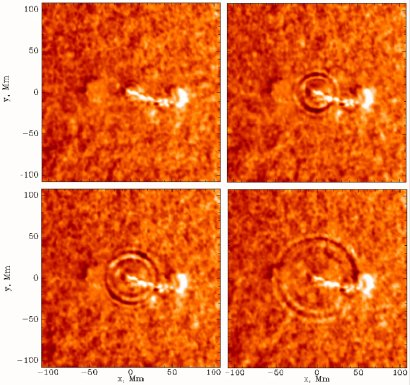
\includegraphics[width=0.5\textwidth]{sunquake.jpg}
\caption{Din\'amica de las ondas expansivas asociadas al primer sismo solar ocurrido el 9 de Julio de 1996 y reportado por \cite{kz1998}.}
\label{fig:sunquake}
\end{center}
\end{wrapfigure}

Las fulguraciones son eventos din\'amicos que involucran cambios significativos en la configuraci\'on del campo magn\'etico coronal. La consecuencia m\'as inmediata es el colapso del bucle coronal hacia una configuraci\'on m\'as estable (m\'as horizontal). Si este proceso se lleva a cabo con la suficiente rapidez podr\'ia llegar a generar trabajo mec\'anico sobre la superficie solar, y por ende, podr\'ia ser un buen candidato en la consideraci\'on de la generaci\'on de la fuente de se\~nales ac\'usticas.  Esta din\'amica posible fue bautizada como el {\it McClymont jerk} por \cite{Hudson2008}. Lo interesante de esta propuesta es que se aleja de hip\'otesis de que es la interacci\'on de las part\'iculas incidentes el detonante de ondas s\'ismicas; sin embargo, a\'un hoy en d\'ia es un tema de \'algida discusi\'on en los diferentes eventos que se celebran en torno a estos temas.\\

?`Cu\'al de todas estas propuestas resulta ser la m\'as eficiente y adecuada para describir el proceso mediante el cual se deposita la energ\'ia necesaria para la generaci\'on del sismo? Es una pregunta que es muy dif\'icil de responder y que solo las observaciones, cada vez de mayor calidad, podr\'an dar luz al respecto. Quiz\'as todo se trate de una soluci\'on salom\'onica en la que dependiendo de las condiciones f\'isicas que definen la prefulguraci\'on uno o varios de estos mecanismos pueden dominar el efecto de generar la fuente ac\'ustica. En el desarrollo que se presenta aqu\'i trabajamos sobre la hip\'otesis de que es justamente el jet de part\'iculas incidentes el mecanismo sobre el cual se podr\'ia asociar la generaci\'on de uno de estos {\it sunquakes}; pero hemos de establecer la forma en que se deben acelerar estas part\'iculas (electrones) que en nuestro caso ser\'a siguiendo una din\'amica estoc\'astica.\\

\section*{M\'etodo de limpieza de observaciones hechas desde tierra}
\addcontentsline{toc}{section}{M\'etodo de limpieza de observaciones hechas desde tierra}

Despu\'es de que \cite{kz1998} reportaran el primer ``{\it tsunami}'' solar, muchos otros cient\'ificos centraron su atenci\'on en tratar de encontrar m\'as eventos como este asociados a fulguraciones solares muy energ\'eticas, con el \'animo de tratar de dar una explicaci\'on f\'isica a la generaci\'on de la fuente s\'ismica mediante un acercamiento m\'as bien estad\'istico. En esta direcci\'on, \cite{detal2006a} desarrollaron una prospecci\'on sobre las fulguraciones m\'as energ\'eticas que ocurrieron durante el m\'aximo del ciclo solar 23 encontrando cerca de 13 eventos s\'ismicos. Para hacer esta inspecci\'on, ellos hicieron uso de las im\'agenes obtenidas por la red de telescopios en tierra GONG++ y aplicaron la t\'ecnica de {\it holograf\'ia heliosismol\'ogica} descrita anteriormente. Sin embargo, y como es bien conocido por todos los astr\'onomos observacionales, el hacer observaciones desde tierra implica tener que considerar los efectos que  tiene la turbulencia atmosf\'erica sobre las im\'agenes obtenidas. En el caso solar esto no es una excepci\'on, y m\'as teniendo en cuenta que para poder distinguir las ondas que se propagan sobre la superficie solar se necesita una resoluci\'on espacial alta en las im\'agenes, de al menos unos tres segundos de arco, adem\'as de un alto contraste regido por la raz\'on se\~nal ruido que para el caso de los {\it sunquakes} es del orden de $\sim 10$, en im\'agenes filtradas por frecuencia, t\'ipicamente centradas en 5 mHz con un pasabandas de 2 mHz \citep[]{kz2006c}. Esta red de observatorios nos ha provisto de fotogramas, Dopplergramas y magnetogramas del Sol calmo de calidad muy alta, pero la limitaci\'on que tiene a la hora de analizar im\'agenes de regiones activas es justamente la consecuencia de la turbulencia atmosf\'erica sobre la imagen final integrada en un minuto de tiempo (imperfecciones por ``{\it seeing}''). En Sol calmo las variaciones debidas a la turbulencia no son percibidas apreciablemente pues no hay una se\~nal fuerte sobre la que puedan influir de sobremanera. Sin embargo, cuando hay un gradiente alto en las intensidades registradas, como es el caso de una regi\'on activa, se genera un ruido que altera las se\~nales s\'ismicas que se quieren analizar haciendo que el implementar los m\'etodos heliosismol\'ogicos sobre las regiones activas se vuelva algo impr\'actico a primera vista.

\subsection*{Algoritmo param\'etrico de correci\'on por turbulencia (PASCAL)}
\addcontentsline{toc}{subsection}{Algoritmo param\'etrico de correci\'on por turbulencia (PASCAL)}

\cite{Lindsey2008} han ideado un algoritmo que aplicado sobre las im\'agenes terrestres obtenidas con GONG++, es capaz de distinguir una se\~nal s\'ismica sobre el ruido de la imagen producto de la turbulencia. Este m\'etodo es aplicable a observaciones que han sido integradas por un periodo de tiempo largo comparado con el tiempo caracter\'istico del ``{\it seeing}'' ($\sim 10$ ms). Teniendo en cuenta que la cadencia de los instrumentos de esta red es de {\bf un minuto}, este m\'etodo resulta ser adecuado a fin de ``limpiar'' las im\'agenes crudas que salen del telescopio siempre y cuando se tenga un excelente control sobre el guiado (``{\it traking}'') de las im\'agenes, lo cual para el caso del Sol se puede hacer muy bien con ayuda del limbo solar.\\

Aunque este m\'etodo de limpieza ha sido aplicado a una cantidad apreciable de estudios heliosismol\'ogicos \citep{detal2006,mo2008a,mo2008b,mo2008d,martinez-oliveros2009,matthews2011,zharkov2011}, no se le ha acu\~nado a\'un un t\'ermino para referirse a este m\'etodo en la literatura. Se ha aprovechado este trabajo y un art\'iculo que est\'a en preparaci\'on para postular el nombre sugerido por {\it Charles Lindsey}: {\bf PASCAL} que son las siglas en ingl\'es de ``{\it {\bf PA}rametric {\bf S}mearing {\bf C}orrection {\bf AL}gorithm}''. Este m\'etodo supone que despu\'es de un minuto de integraci\'on (que es la cadencia t\'ipica de los instrumentos de GONG) las perturbaciones atmosf\'ericas pueden ser consideradas como isotr\'opicas, cosa que facilita mucho el planteamiento de un tratamiento pr\'actico sobre las im\'agenes y que no est\'a lejos de la realidad pues un minuto de integraci\'on significa unas dos mil variaciones de la imagen que se registra debido al {\it seeing} atmosf\'erico.\\

Supongamos que $I(\mathbf{r})$ representa la intensidad real del objeto sobre la imagen cruda que se obtiene del instrumento, mientras que $I'(\mathbf{r})$ representa la intensidad observada (es decir la imagen real convolucionada con el ruido atmosf\'erico integrado en un minuto). $S(\mathbf{r})$ representar\'a la funci\'on (isotr\'opica) de la perturbaci\'on atmosf\'erica. Todas estas cantidades dependen de $\mathbf{r}$ que es la ubicaci\'on de un punto sobre la imagen cruda. De esta manera se tiene que

\begin{align}
I'&=(S*I)\\
SI&=(S*I).
\end{align}

Este operador de perturbaci\'on,$S$, debe contener los efectos que la atm\'osfera tiene sobre las im\'agenes en su totalidad.

\begin{wrapfigure}[30]{l}{0.65\textwidth}
\begin{center}
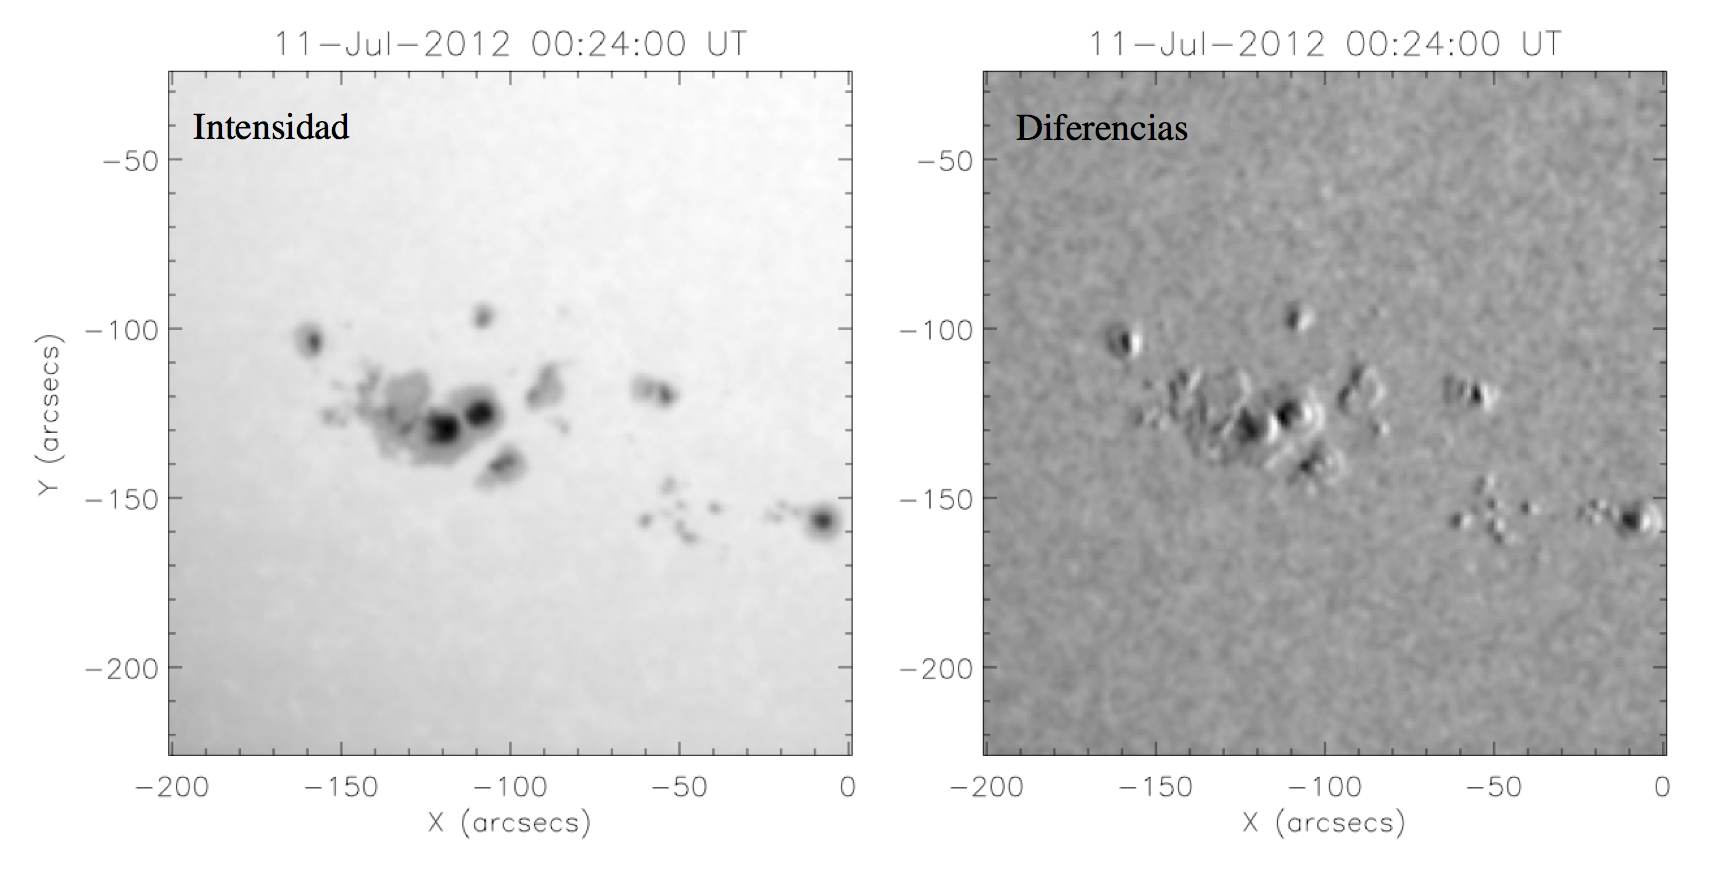
\includegraphics[width=0.64\textwidth]{Diff_gong.png}
\caption{Regi\'on activa NOAA 11520 que fue visible desde tierra desde el 6 de Julio hasta el 17 de Julio de 2012. Esta mancha solar se caracteriz\'o por ser tan grande que fue posible observarla con los filtros adecuados pero sin instrumentos de aumento en el marco de lo que fue la {\it International Summer School - Solar Astrophysics: Modern Trends and Techniques} realizada en Bogot\'a. {Izquierda}: Imagen en intensidad tomada por GONG++ el 11 de Julio de 2012 a las 00:24 UT. {Derecha}: Diferencia entre la imagen de la izquierda y la registrada por GONG++ al minuto siguiente (00:25 UT). Es claramente apreciable como los efectos de {\it seeing} atmosf\'erico tienen mayor incidencia sobre las regiones activas que sobre el Sol-calmo. Im\'agenes de diferencias, como la que se muestra aqu\'i, son usada en el m\'etodo {\bf PASCAL} para caracterizar las perturbaciones presentes en la im\'agen minuto a minuto.}
\label{fig:diff_gong}
\end{center}
\end{wrapfigure}

Estos efectos se pueden representar en dos din\'amicas b\'asicas. Una traslaci\'on estoc\'astica de la regi\'on de inter\'es, que aqu\'i se representa mediante un vector  desplazamiento $\vec{\alpha}$ definido sobre el plano de la im\'agen, y una deformaci\'on (difusi\'on) de la imagen debido a la diferencia de los caminos \'opticos de los rayos provenientes del objeto de ciencia extendido, que en nuestro caso es el disco solar, y que supondremos se caracteriza por un par\'ametro $\beta$. De esta manera el operador $\hat{S}$ se puede expresar como la suma de un t\'ermino convetivo y un t\'ermino difusivo que act\'uan sobre la se\~nal real:

\begin{align}
\hat{S}(\mathbf{r})=\hat{1}-\vec{\alpha}\cdot\vec{\nabla} + \beta\nabla^2
\end{align}

Para poder aplicar el m\'etodo se hacen dos suposiciones adicionales: Se supone que las perturbaciones generadas sobre la imagen producto del {\it seeing} atmosf\'erico son isotr\'opicas y que el tama\~no de estas son significativamente m\'as peque\~nas que el tama\~no del objeto de ciencia. Gracias a estas suposiciones podemos agrupar el t\'ermino convectivo dentro del t\'ermino difusivo y tratar la perturbaci\'on como un efecto que act\'ua de la forma $\hat{S}=\hat{1} + \beta'\nabla^2$, de manera que aplicado sobre la imagen {\it real} tenemos:

\begin{align}\label{operadorS}
\hat{S}I(\mathbf{r})&= I + \beta'(\mathbf{r})\nabla^2I(\mathbf{r})\\
I'(\mathbf{r})&= I(\mathbf{r}) + \beta'(\mathbf{r})\nabla^2I(\mathbf{r})\\
\Delta I(\mathbf{r})&=\beta'(\mathbf{r})\nabla^2I(\mathbf{r}).
\end{align}

En un periodo de tiempo del orden de un par de horas podemos suponer que $\Delta I(\mathbf{r})=[I'(\mathbf{r})-I(\mathbf{r})]\approx [I'_{(t_i+1\,\text{min})}(\mathbf{r})-I_{t_i}'(\mathbf{r})]$, de manera que im\'agenes de la diferencia entre dos fotogramas consecutivos tomados por GONG++, como la que se muestra en la figura \ref{fig:diff_gong}, representan muy bien el t\'ermino difusivo $\beta'\nabla^2 I_{t_i}(\mathbf{r})$. El algoritmo que \cite{Lindsey2008} desarrollaron lo que hace es justamente ajustar las im\'agenes de diferencias a un laplaciano de la im\'agen precedente y calcular de esta manera los coeficientes $\beta'(\mathbf{r})$ para cada p\'ixel de la imagen de ciencia y con la cadencia del instrumento, un minuto. De esta manera la tarea se reduce a tener que resolver num\'ericamente una ecuaci\'on de {\it Poisson} en cada punto de la imagen a la cual previamente se le ha aplicado una proyecci\'on {\it Postel} para garantizar que se est\'a trabajando en un espacio homog\'eneo e isotr\'opico. Para resolver la ecuaci\'on de {\it Laplace}, \cite{Lindsey2008} aplicaron el m\'etodo de {\it diferencias finitas} inicialmente con un esquema de {\bf 5 puntos} para la descomposici\'on del {\it Laplaciano} que parece en la ecuaci\'on de {\it Poisson}. 

\subsection*{Algoritmo num\'erico para el c\'alculo del laplaciano de una funci\'on bidimensional}
\addcontentsline{toc}{subsection}{Algoritmo num\'erico para el c\'alculo del laplaciano de una funci\'on bidimensional}

\begin{wrapfigure}[24]{r}{0.5\textwidth}
\begin{center}
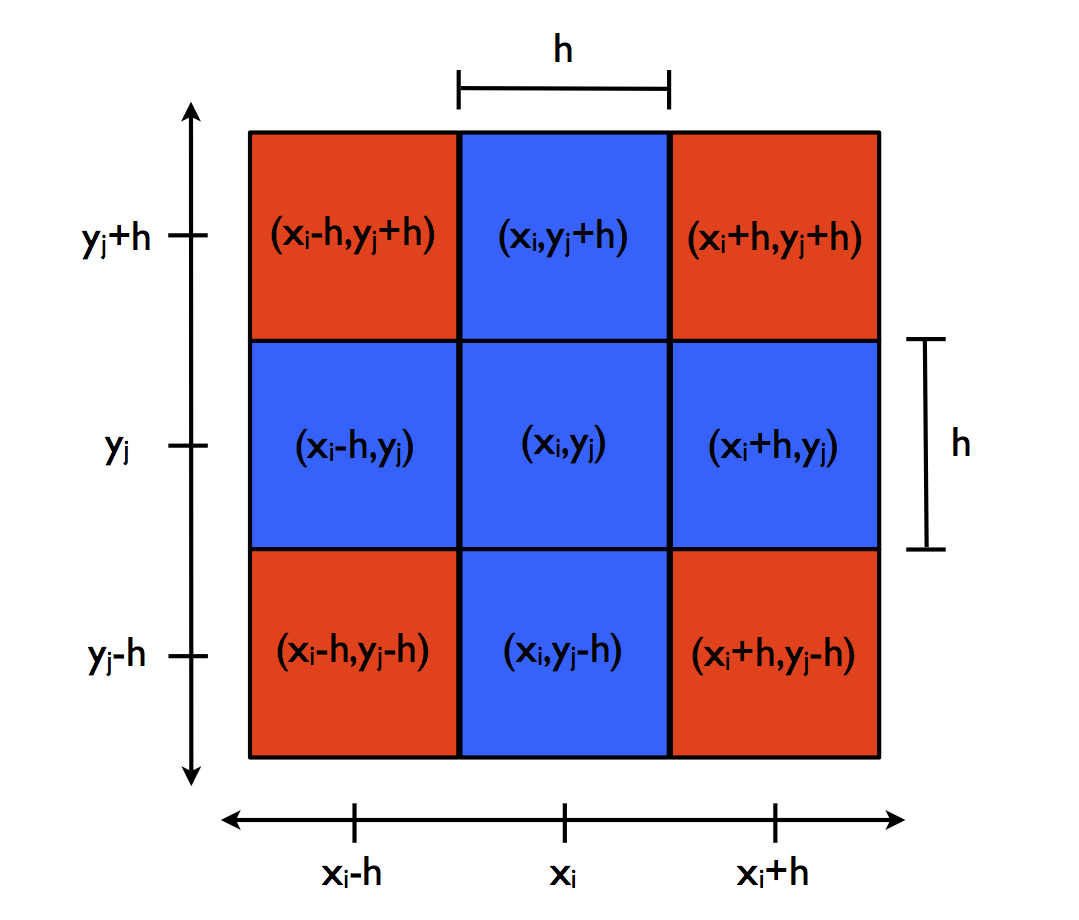
\includegraphics[width=0.52\textwidth]{9puntos.png}
\caption{Ilustraci\'on de los primeros (cuadros azules) y segundos (cuadros rojos) vecinos de una celda que pertenece a una grilla a la cual se le piensa aplicar un m\'etodo num\'erico tales como el de {\it Lattice Boltzmann} o el de diferencias finitas.}
\label{fig:9puntos}
\end{center}
\end{wrapfigure}

Modernamente las im\'agenes solares se registran en arreglos bi-dimensionales finitos de p\'ixeles en c\'amaras CCDs; usualmente, estas c\'amaras tienen escalas iguales en ambos ejes, los cuales denotamos como ejes $x$, $y$. Al trabajar sobre estos arreglos podemos expresar al laplaciano como 

\begin{align}
\nabla^2I(\mathbf{r})=\nabla^2I(x,y)\approx f(x,y),
\end{align}

\noindent en donde se define $f(x,y)=\frac{\Delta I(x,y)}{\beta'(x,y)}$, asumiendo adem\'as que las variables cartesianas $x$, $y$ son linealmente independientes. El c\'alculo num\'erico del laplaciano en un punto interior del fotograma bajo estudio tiene ocho puntos vecinos. Existen dos posibilidades sencillas del c\'alculo del laplaciano; uno que contempla los p\'ixeles en el vecindario inmediato de columna y fila, a los cuales llamaremos de aqu\'i en adelante los primeros vecinos, y que se ilustran en azul en la figura \ref{fig:9puntos}. El otro m\'etodo considera al vecindario inmediato completo, es decir, tanto los cuadros azules como rojos de la figura \ref{fig:9puntos}. Al laplaciano calculado en el primero de los casos lo llamaremos el {\it laplaciano de 5 puntos}. Este se puede expresar como:

\begin{align}\label{eq:lap5}
\nabla^2I(x_i,y_j)&\approx I(x_i+h,y_j)+I(x_i-h,y_j)\\\nonumber
&+I(x_i,y_j+h)+I(x_i,y_j-h)\\\nonumber
&-4I(x_i,y_j)=h^2f(x_i,y_j),
\end{align}

\noindent en donde $h$ es el tama\~no del lado del cuadrado de un p\'ixel que por razones de simplicidad en la implementaci\'on del m\'etodo num\'erico se tom\'o como uno. Esta forma de calcular el laplaciano es haciendo uso de los primeros vecinos del p\'ixel ubicado en $(x_i,y_j)$ obteniendo una precisi\'on de segundo orden en $h$. Si se quiere hacer este mismo c\'alculo pero incluyendo adem\'as a los segundos vecinos del p\'ixel evaluado  (cuadros rojos de la figura \ref{fig:9puntos}), entonces se procede implementando lo que se conoce como el c\'alculo del laplaciano con {\bf 9 puntos}, de forma que se tiene \citep{vooren1967}:

\begin{align}
&\nabla^2I(x_i,y_j)=f(x_i,y_j),\\\nonumber
&I(x_i+1,y_j+1)+I(x_i+1,y_j-1)+I(x_i-1,y_j+1)+I(x_i-1,y_j-1)+\\\nonumber
&+4\,[I(x_i+1,y_j)+I(x_i-1,y_j)+I(x_i,y_j+1)+I(x_i,y_j-1)]-20\,I(x_i,y_j)=6f(x_i,y_j).
\end{align}

Una vez hallados los $f(x_i,y_j)$ sobre toda la grilla, es posible determinar el valor de los $\beta'$ para cada p\'ixel mediante $\beta'(x_i,y_j,t_k)=\frac{\Delta I(x_i,y_j,t_k)}{f(x_i,y_j,t_k)}$, y de esta manera construir el operador $\hat{S}$ definido en (\ref{operadorS}) para finalmente aplicarlo como m\'etodo de limpieza a la totalidad de las im\'agenes. Todos los trabajos desarrollados hasta este momento en los que se desarrollan an\'alisis heliosismol\'ogicos usando im\'agenes de la red GONG han 

\begin{wrapfigure}[27]{r}{0.55\textwidth}
\begin{center}
\subfloat{
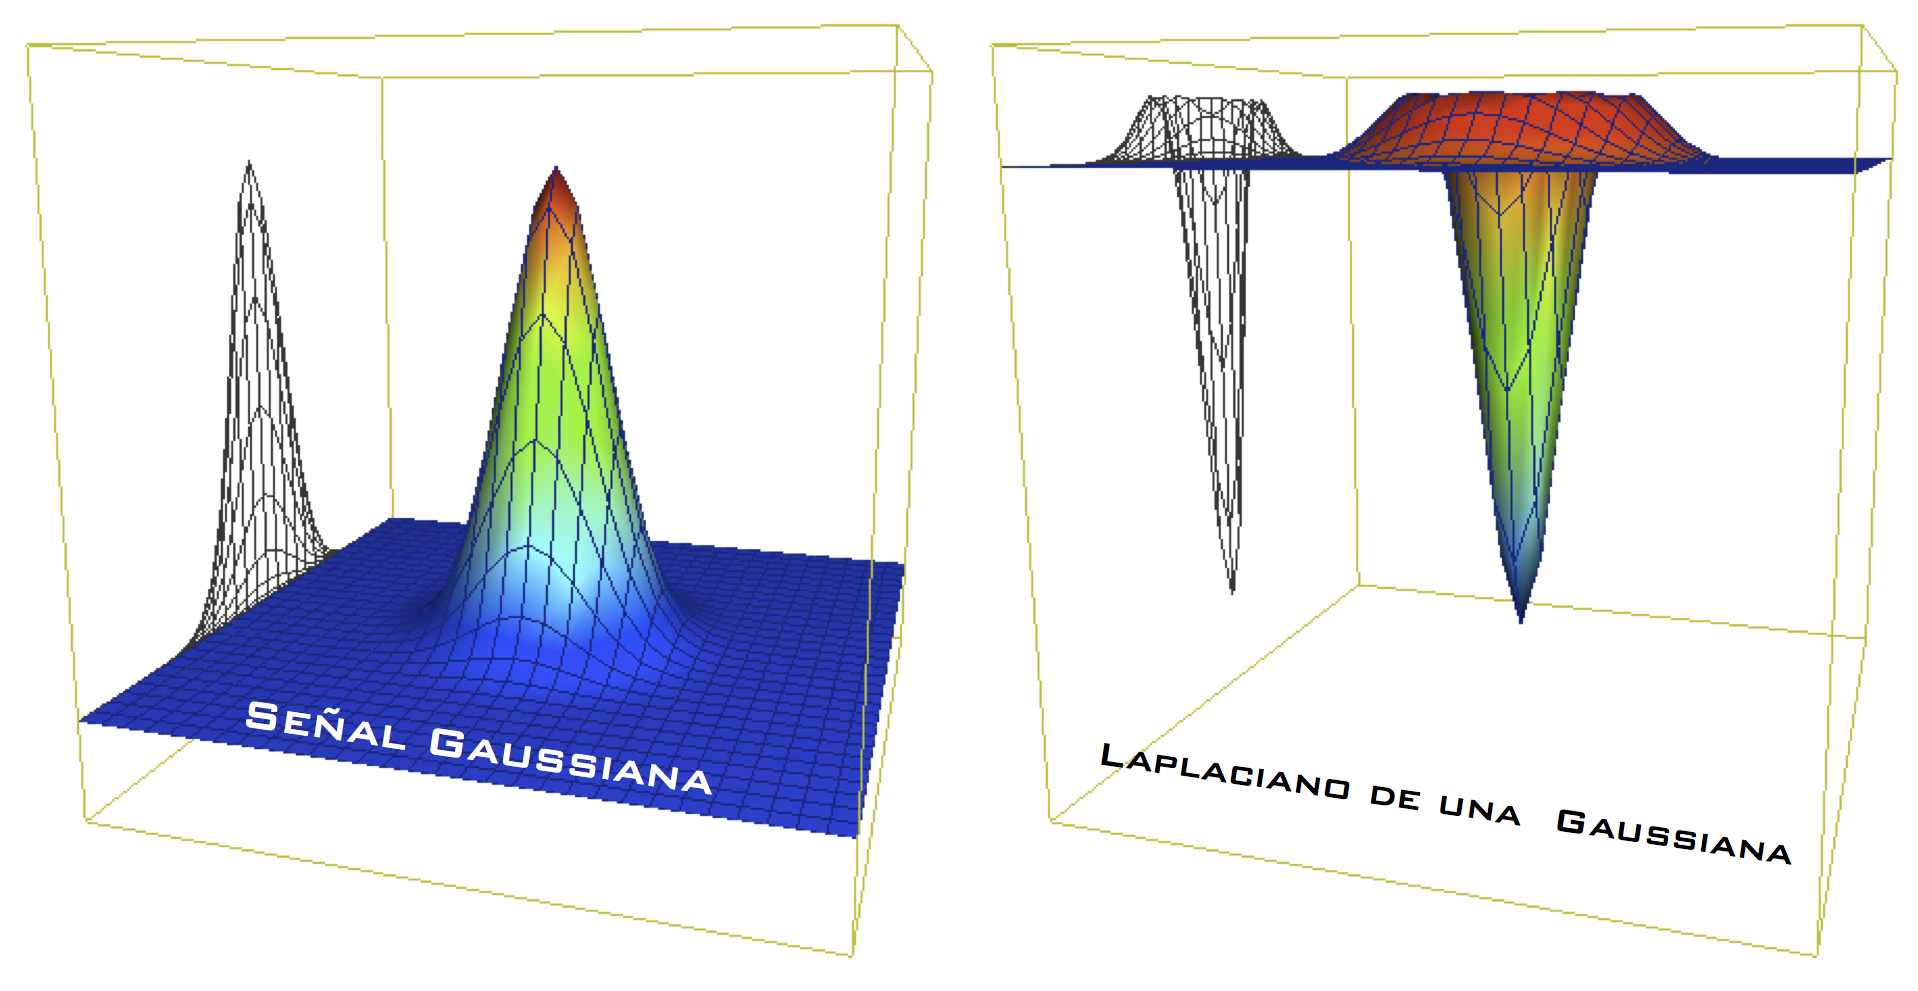
\includegraphics[width=0.55\textwidth]{gauss.png}
}\\[20pt]
\subfloat{
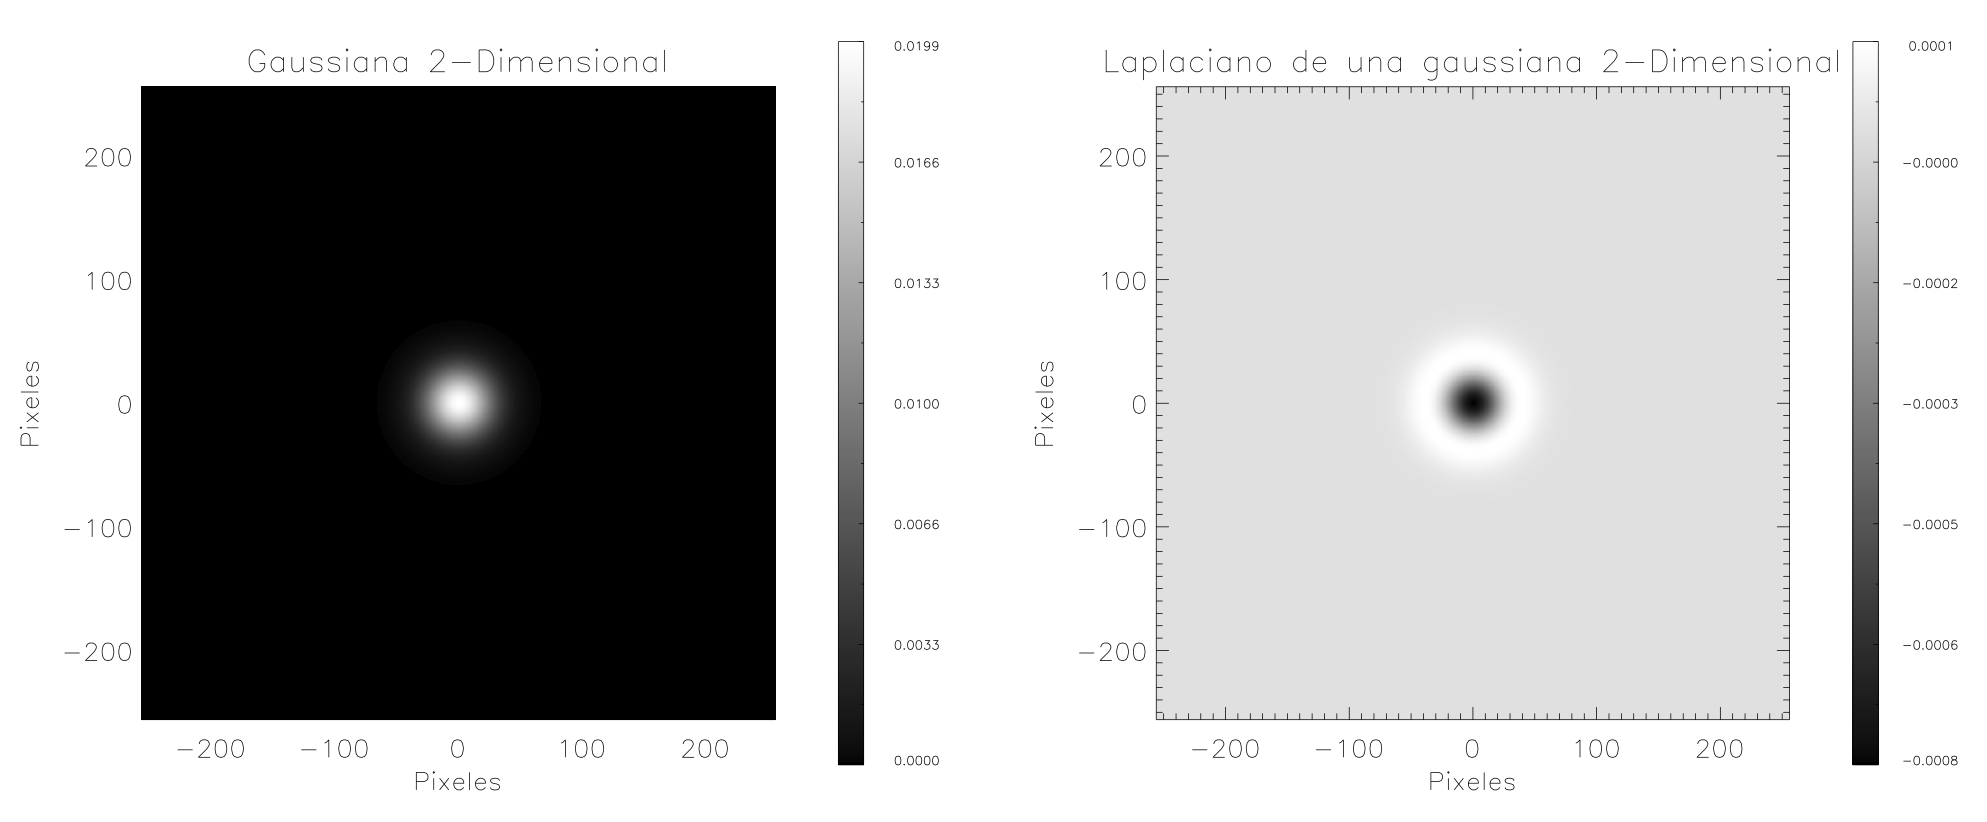
\includegraphics[width=0.55\textwidth]{gauss_lap_teo.png}
}
\caption{{\it Izquierda:} Se\~nal gaussiana bi-dimensional que sigue la expresi\'on dada por la ecuaci\'on  (\ref{eq:gauss}) con un $\sigma=0.8$. {\it Derecha}: Laplaciano de la gaussiana construida siguiendo la forma funcional dada en (\ref{eq:lapgauss}). {\it Arriba:} Visualizaci\'on en 3D. {\it Abajo:} Visualizaci\'on en 2D con escala de grises.}
\label{fig:gauss}
\end{center}
\end{wrapfigure}


\noindent implementado el m\'etodo PASCAL calculando un laplaciano de 5 puntos \citep{detal2006,Lindsey2008,mo2008a,mo2008b,mo2008d,martinez-oliveros2009,matthews2011,zharkov2011}. En este trabajo tomamos los c\'odigos que contienen el m\'etodo PASCAL trabajados por {\it Charles Lindsey} y los modificamos de tal manera que el ajuste del laplaciano se hiciera mediante el algoritmo de 9 puntos con el fin de aplicarlo sobre un evento s\'ismicamente activo, que se conociera muy bien, y poder compararlo con el m\'etodo que usa 5 puntos en aras de encontrar alguna diferencia, el cual es el objetivo de este cap\'itulo. Para poder comparar estos dos algoritmos, lo primero que se debe hacer es aplicarlos sobre una se\~nal conocida y examinar la precisi\'on asociada a cada uno. La primera prueba que se desarrolla es la aplicaci\'on de estos algoritmos sobre una se\~nal {\it gaussiana}, cuya expresi\'on en dos dimensiones es

\begin{align}\label{eq:gauss}
G(x,y)=\frac{1}{\sqrt{2\pi\sigma^2}}\exp\left[-\frac{x^2+y^2}{2\sigma^2}\right],
\end{align} 

\noindent y de la cual es posible conocer te\'oricamente su laplaciano

\begin{align}\label{eq:lapgauss}
\nabla^2G(x,y)=-\frac{1}{\pi\sigma^2}\left(1-\frac{x^2+y^2}{2\sigma^2}\right)\exp\left(-\frac{x^2+y^2}{2\sigma^2}\right).
\end{align}

\begin{SCfigure}
%\begin{center}
\subfloat[]{
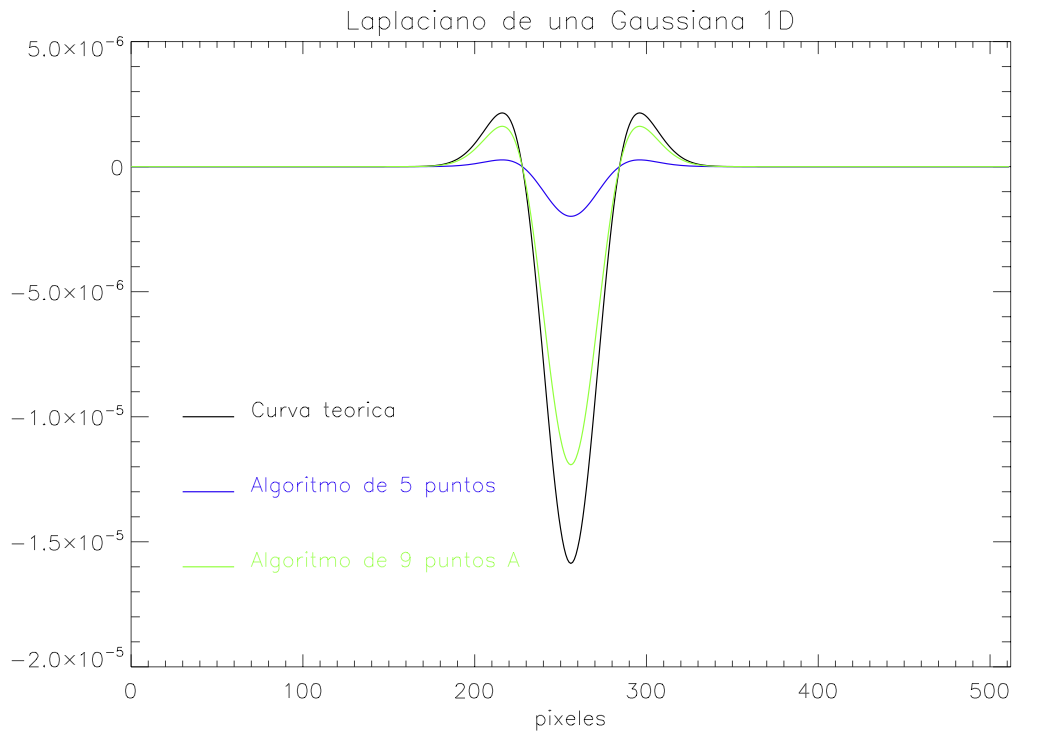
\includegraphics[width=0.35\textwidth]{Laplacian_1D.png}
}
\subfloat[]{
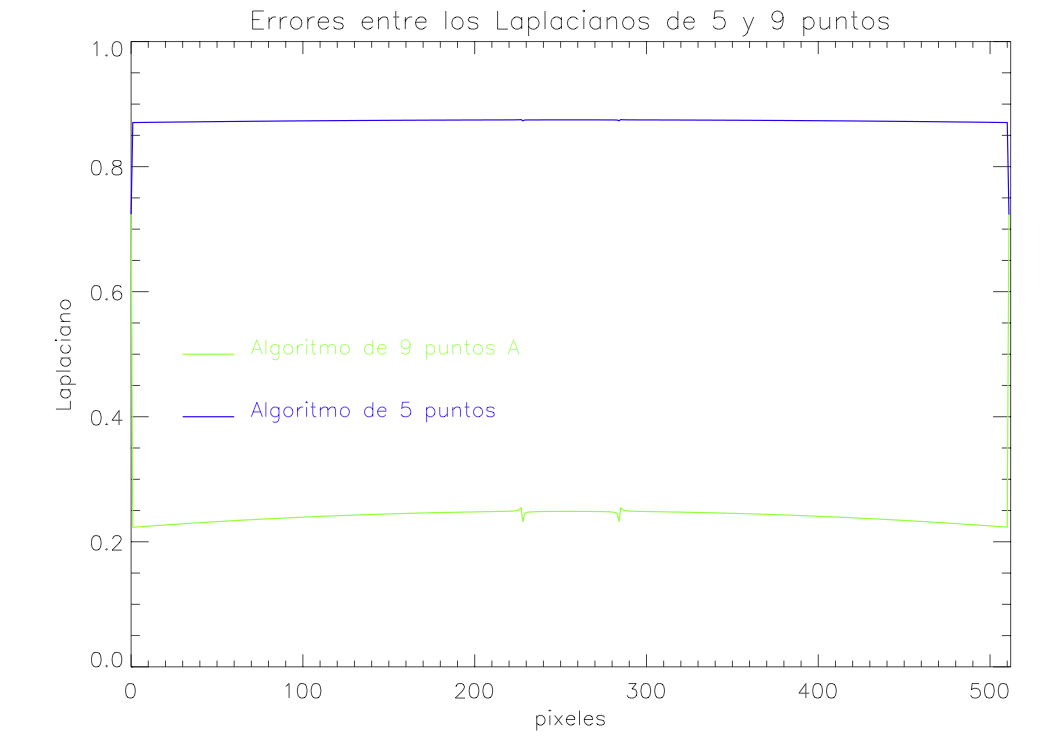
\includegraphics[width=0.35\textwidth]{Laplacian_1D_errores.png}
}
\caption{(a) Comparaci\'on del c\'alculo num\'erico del laplaciano de la se\~nal gaussiana de la figura \ref{fig:gauss} usando los dos algoritmos, el de cinco (curva azul) y el de nueve (curva verde) puntos, y su comparaci\'on con su curva te\'orica (curva negra). (b) Errores de cada uno de los dos m\'etodos con respecto al valor te\'orico.}
\label{fig:perfiles}
%\end{center}
\end{SCfigure}



\noindent En la figura \ref{fig:gauss} se presenta una visualizaci\'on en 3D (arriba) tanto de la se\~nal gaussiana como la de su laplaciano, de acuerdo con las ecuaciones (\ref{eq:gauss}) y (\ref{eq:lapgauss}) respectivamente, con proyecciones planas correspondientes a la variaci\'on de intensidad versus la distancia al centro de la gaussiana, y en la parte inferior de la figura  se han representado las visualizaciones respectivas en un plano de imagen. Para poder hacer una primera comparaci\'on entre los dos m\'etodos usados para calcular num\'ericamente el laplaciano, se hace un corte horizontal que contiene al centro de imagen plana del laplaciano, en nuestro caso al centro de la imagen de la figura \ref{fig:gauss} en la parte baja a la derecha. De esta manera se obtuvieron los perfiles correspondientes al caso te\'o rico como a los dos casos calculados con base en los laplacianos de cinco y de nueve puntos. En la figura \ref{fig:perfiles} la l\'inea negra da cuenta de la curva te\'orica calculada para el laplaciano de una se\~nal gaussiana bidimensional, mientras que las l\'ineas azul y verde representan el c\'alculo num\'erico desarrollado sobre la gaussiana que se muestra en la parte baja de la figura \ref{fig:perfiles} haciendo uso de los m\'etodos de cinco y nueve puntos respectivamente. Claramente, el ajuste con nueve puntos se acerca mucho mejor a la curva te\'orica de lo que lo hace el algoritmo con cinco puntos, como era de esperarse. En la parte (b) de la figura \ref{fig:perfiles} se muestran, adem\'as, los errores porcentuales punto a punto de cada uno de los dos m\'etodos; en dicha gr\'afica se puede apreciar la mejor precisi\'on del m\'etodo de nueve puntos. Ahora bien, una funci\'on gaussiana bidimensional es homog\'enea e isotr\'opica con respecto a su punto central, pero, ?`qu\'e pasar\'ia si ahora aplicamos estos dos mismos m\'etodos de c\'alculo num\'erico sobre una funci\'on que no tenga este par de caracter\'isticas? Para dar respuesta a esta pregunta, se plantea un tratamiento previo a la se\~nal gaussiana que se dividir\'a en dos pasos. El primero consta en amplificar la funci\'on gaussiana a lo largo del eje $x$ en un factor 2 y a comprimirla a lo largo del eje $y$ en un factor $1/2$, y como segundo paso, se calcula nuevamente su laplaciano, tanto te\'orica como num\'ericamente. El resultado es algo como lo que se muestra en la figura \ref{fig:gaussaplastada}. En esta figura se muestra la funci\'on gaussiana achatada (a), su respectivo laplaciano te\'orico (b), el laplaciano num\'erico calculado mediante el algor\'itmo de cinco puntos (c), y el laplaciano num\'erico calculado mediante el algor\'itmo de nueve puntos (d). All\'i se evidencia un diferencia notoria entre el laplaciano te\'orico y los laplacianos num\'ericos, hacia los extremos de la funci\'on a lo largo del eje horizontal.


\begin{figure}[ht!]
\begin{center}
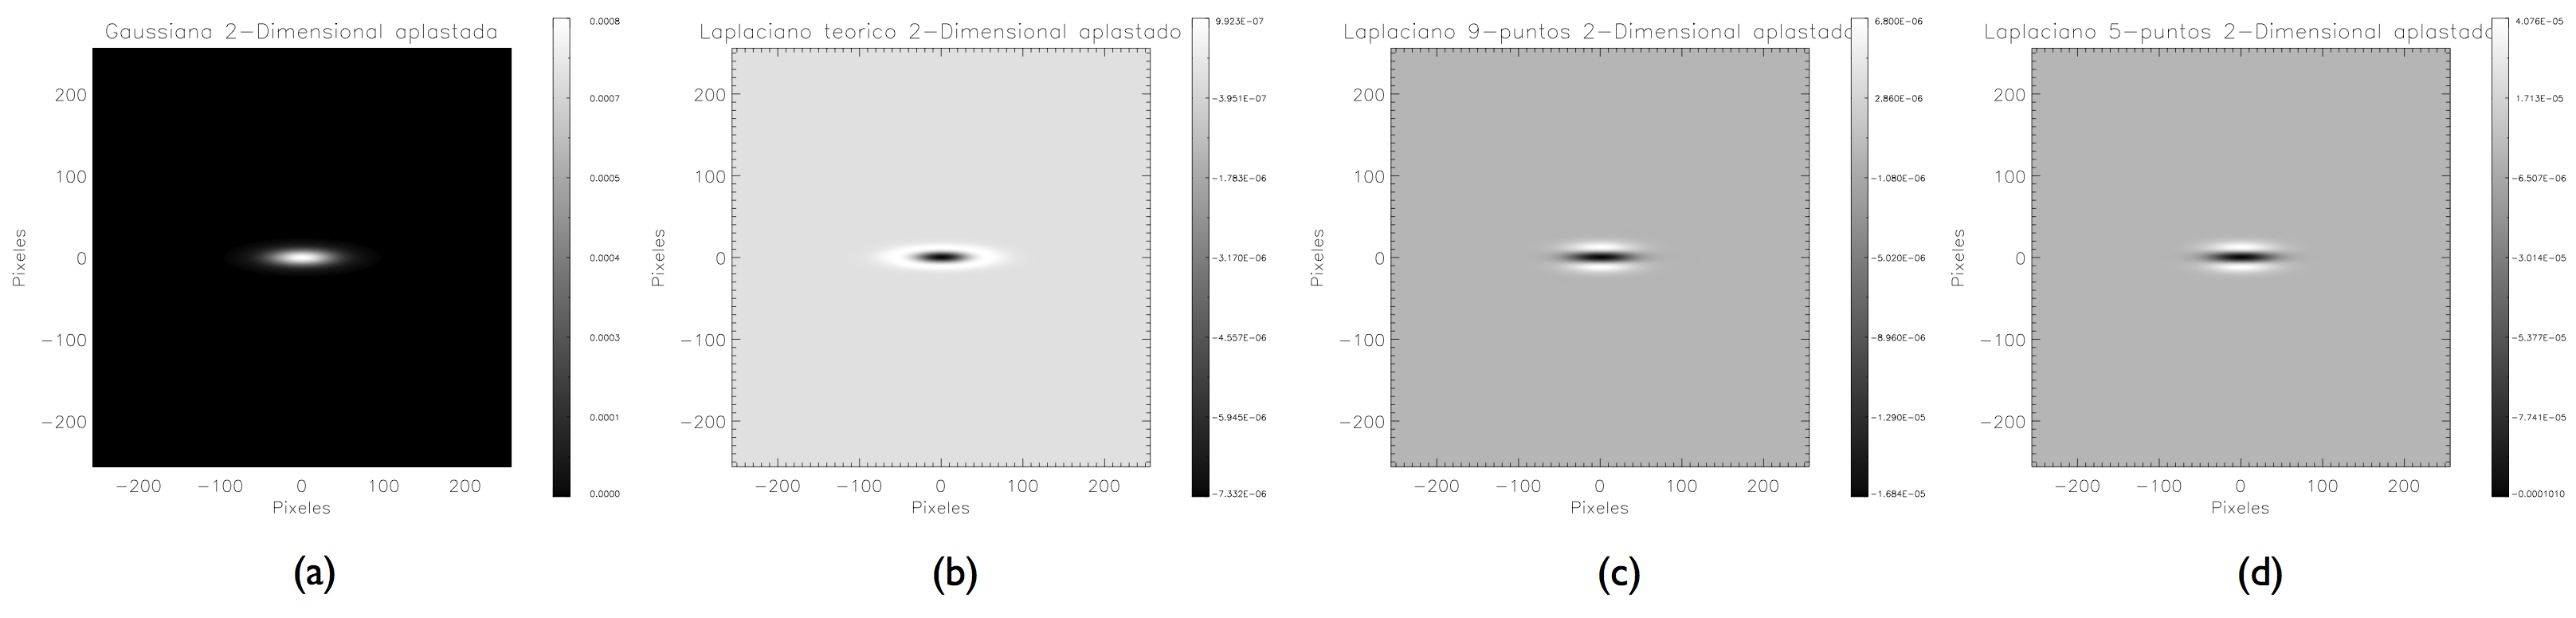
\includegraphics[width=1.0\textwidth]{aplastada.png}
\caption{{\it (a)} Funci\'on gaussiana bidimensional achatada a lo largo del eje vertical y alargada a lo largo del eje horizontal. {\it (b)} Laplaciano te\'orico de la funci\'on gaussiana de la izquierda calculada mediante la implementaci\'on adecuada de la ecuaci\'on (\ref{eq:lapgauss}). {\it (c)} Laplaciano num\'erico calculado mediante la implementaci\'on del algoritmo de cinco puntos.  {\it (d)} Laplaciano num\'erico calculado mediante la implementaci\'on del algoritmo de nueve puntos.}
\label{fig:gaussaplastada}
\end{center}
\end{figure}


Dicha discrepancia es debida a que los algoritmos que se est\'an usando para el c\'alculo num\'erico del laplaciano son definidos para ser trabajados sobre se\~nales (funciones) {\it homog\'eneas}, y claramente la funci\'on gaussiana achatada de la figura \ref{fig:gaussaplastada}(a) no lo es. Dado este escenario, se ve la necesidad de modificar de alguna manera los algoritmos que calculan el laplaciano de manera que se consideren en ellos las formas inhomog\'eneas de las se\~nales bajo estudio. En esta direcci\'on se propone asignar pesos diferentes a los p\'ixeles vecinos de cada p\'ixel sobre el que se lleva a cabo el c\'alculo num\'erico de manera que se contrarresten los efectos de la geometra\'ia no homog\'enea de la funci\'on.\\


\begin{figure}
\begin{center}
\subfloat[]{
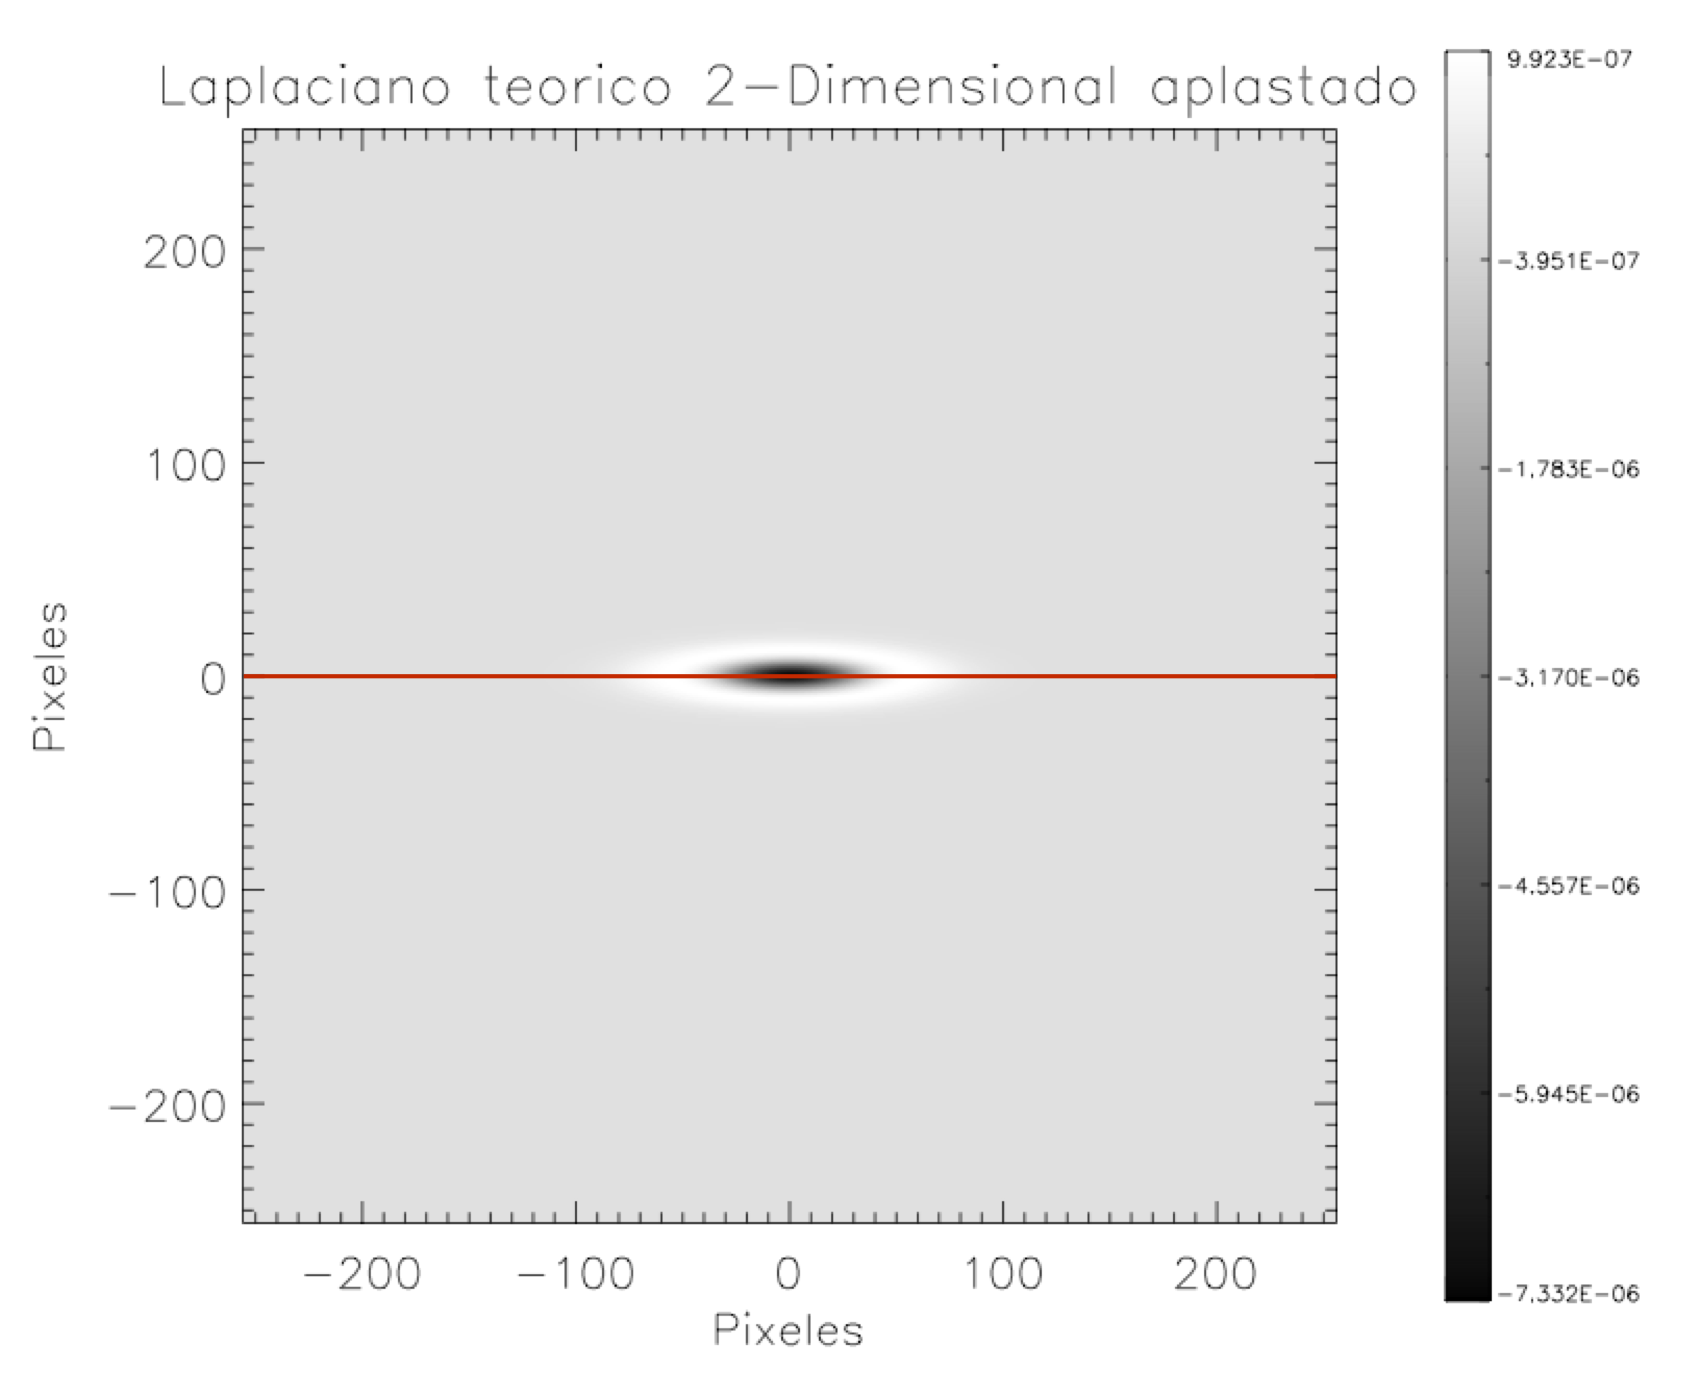
\includegraphics[width=0.3\textwidth]{lapt_aplastada.png}
}
\subfloat[]{
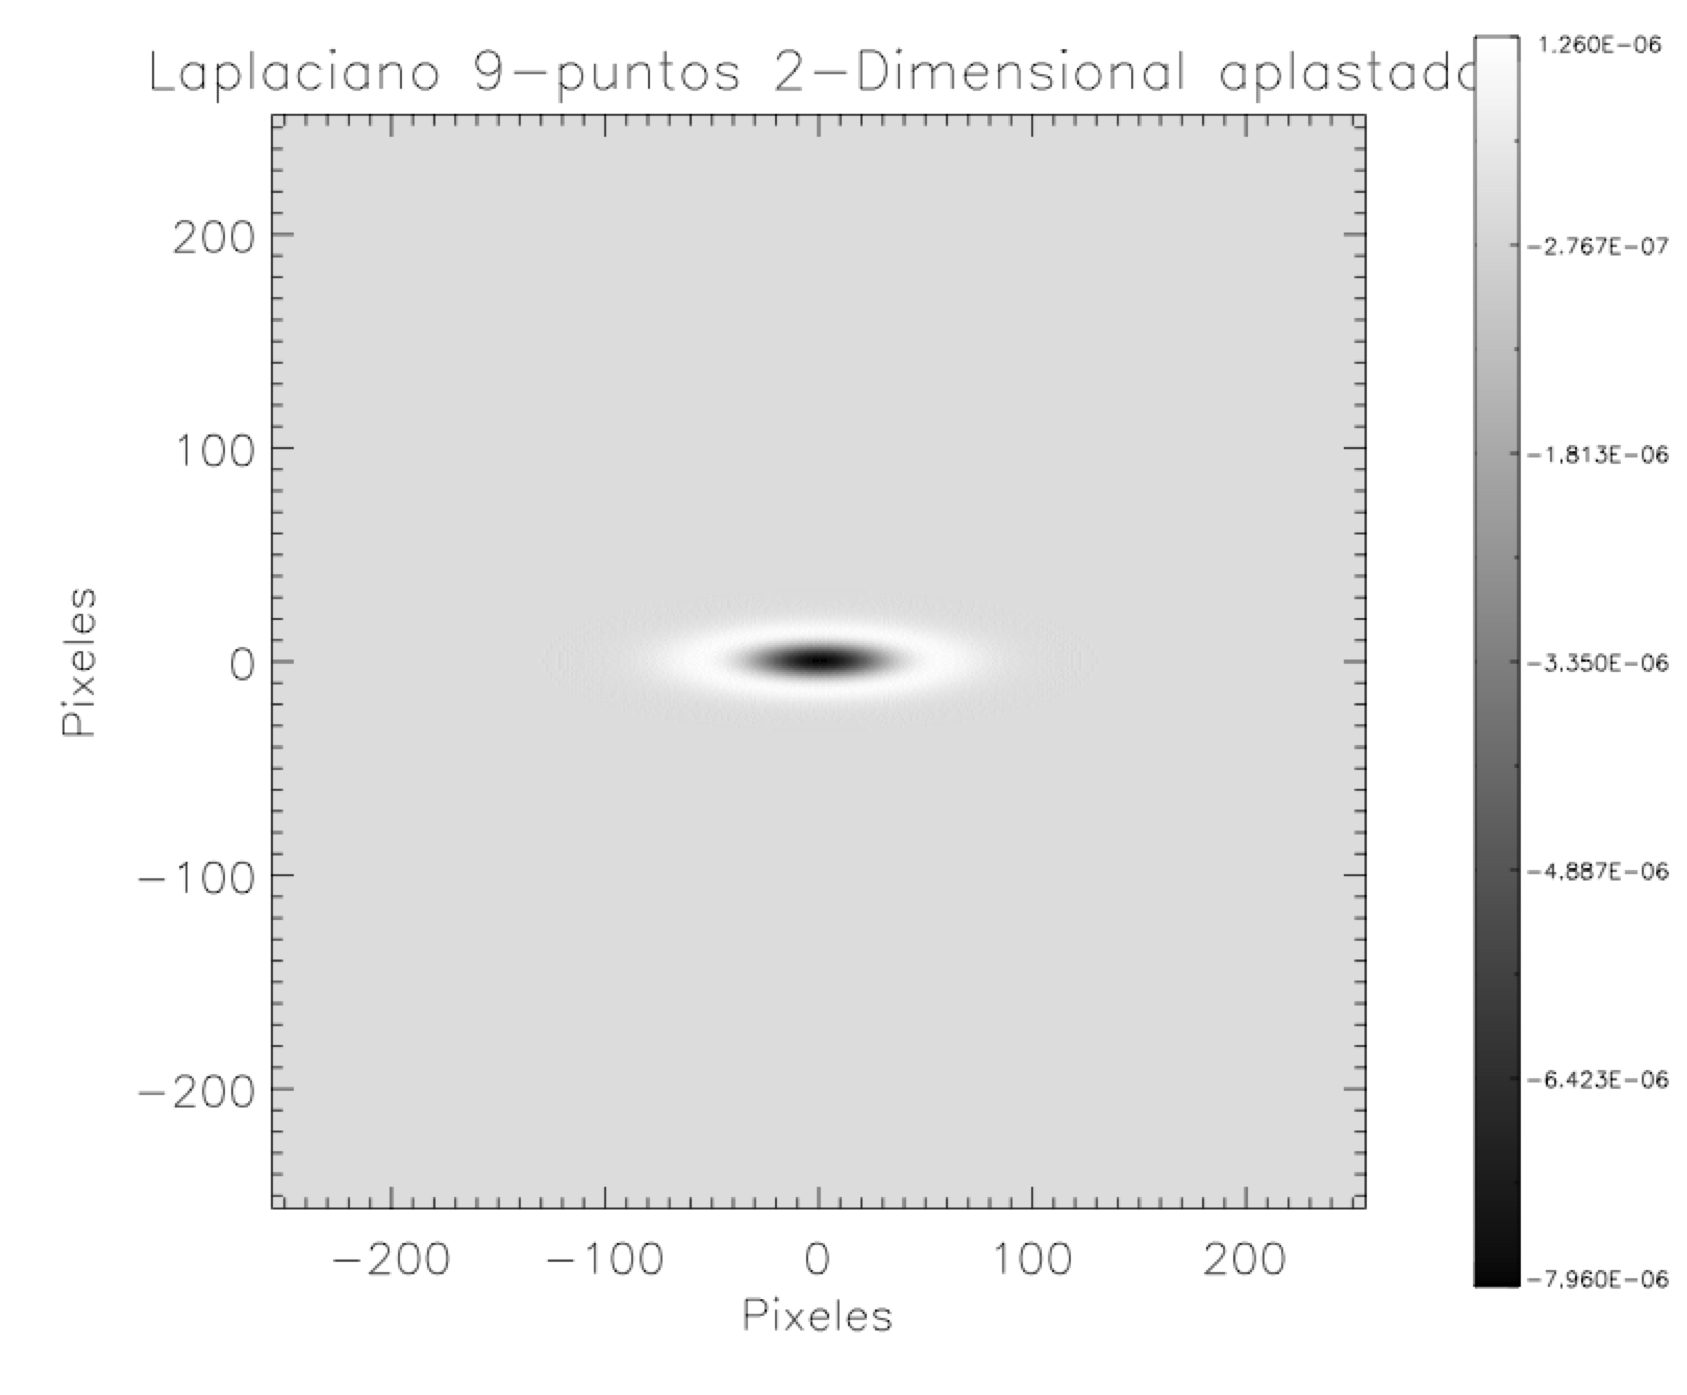
\includegraphics[width=0.3\textwidth]{lap9j_aplastada.png}
}
\subfloat[]{
\includegraphics[width=0.3\textwidth]{Lap_mod_Teo.png}
}
\caption{{\it (a)} Laplaciano te\'orico de la gaussiana achatada de la figura \ref{fig:gaussaplastada}. La l\'inea roja indica la regi\'on escogida para hacer los perfiles que se muestran en (c). {\it (b)} Laplaciano de nueve puntos con pesos asignados por la ecuaci\'on \ref{eq:lapmod} con $\alpha=0.5$, $\beta=2.0$ y $\gamma=0.0$. {\it (c)} Perfiles de comprarci\'on de los dos laplacianos. la curva negra es el perfil te\'orico y la roja es el perfil obtenido mediante el algoritmo de 9 puntos con pesos en sus primeros vecinos. Se error obtiene un error del $15\%$, en promedio, entre las dos curvas.}
\label{fig:lapmod}
\end{center}
\end{figure}


\noindent As\'i, el nuevo algoritmo se expresar\'ia mediante 

\begin{align}\label{eq:lapmod}
\nabla^2I(x_i,y_j)&=f(x_i,y_j),\\\nonumber
f(x_i,y_j)&=\alpha[I(x_i,y_j+1)+I(x_i,y_j-1)-2I(x_i,y_j)]\\\nonumber
&+\beta[I(x_i+1,y_j)+I(x_i-1,y_j)-2I(x_i,y_j)]\\\nonumber
&+\frac{\gamma}{4}[I(x_i+1,y_j+1)-I(x_i-1,y_j+1)-I(x_i+1,y_j-1)+I(x_i-1,y_j-1)],\label{eq:lapmod}
\end{align}


\noindent en donde $\alpha$, $\beta$, $\gamma$ son los par\'ametros escalares que dan peso a los primeros y segundos vecinos, del p\'ixel sobre el que se realiza el c\'alculo, a lo largo del eje horizontal, del eje vertical y de los ejes diagonales respectivamente. Para su implementaci\'on, por ejemplo, en el caso considerado en la figura \ref{fig:gaussaplastada}, un buen ajuste se consigue al definir $\alpha=0.5$, $\beta=2.0$ y $\gamma=0.0$. Un perfil horizontal sobre dicho ajuste con su respectiva comparaci\'on con el valor te\'orico de \'este se muestran en la figura \ref{fig:lapmod}. De esta figura se evidencia una clara mejor\'ia en el ajuste del m\'etodo n\'umerico con la curva te\'orica y se corrobora al hacer el c\'alculo de su error porcentual de un $15\%$ en promedio.\\

Siguiendo con la prueba de funcionalidad del c\'alculo num\'erico del laplaciano, se plantea ahora rotar la funci\'on con respecto al origen coordenado en una cantidad de $45^\circ$ y $315^\circ$ como se muestra en la figura \ref{fig:gausssquezee}. Observe que la l\'inea roja trazada en la figura \ref{fig:lapmod} es la misma que aparece en la figura \ref{fig:gausssquezee}. Este m\'etodo da origen a una se\~nal que emular\'ia a la funci\'on gaussiana vista de perfil, es decir, algo as\'i como si esta proviniera de un lugar en la superficie solar m\'as cerca hacia el limbo del disco solar observado desde la tierra. Esto se hace justamente en busca de evaluar la precisi\'on de cada m\'etodo sobre se\~nales que no necesariamente se hayan presentado en el centro del disco del Sol, pues como es bien sabido una fulguraci\'on solar puede presentarse en cualquier regi\'on sobre el discosolar. Para la se\~nal de la parte superior de la figura \ref{fig:gausssquezee}, la cual ha sido rotada un \'angulo de $45^\circ$, tomamos los par\'ametros $\alpha=1.0$, $\beta=1.0$ y $\gamma=1.6$ en aras de contrarrestar el efecto de la proyecci\'on y de darle un mayor peso a la direcci\'on diagonal inclinada un \'angulo de $45^\circ$ en el sentido antihorario, obteniendo as\'i el laplaciano num\'erico bidimensional que se muestra en la parte izquierda de la figura \ref{fig:lapjc45}. As\'i mismo, sobre la l\'inea roja horizontal, de esta misma figura, se traz\'o el perfil de la gaussiana para verificar de manera unidimensional la calidad de su ajuste. Este perfil se muestra al lado derecho de la figura \ref{fig:lapjc45}. El error promedio de este laplaciano num\'erico no homog\'eneo es del $5\%$ con respecto a la curva te\'orica calculada. Dada la antisimetr\'ia del conjunto de t\'erminos que da cuenta de las contribuciones diagonales en el c\'alculo del laplaciano num\'erico dado por la ecuaci\'on \ref{eq:lapmod}, se espera que para una gaussiana modificada de la misma manera que esta \'ultima que trabajamos pero con una rotaci\'on neta de $315^\circ$ en sentido antihorario los coeficientes que asignan peso a cada p\'ixel de la vecindad inmediata est\'en dados por $\alpha=1.0$, $\beta=1.0$ y $\gamma=-1.6$. Al desarrollar este procedimiento se encuentra algo como lo que se muestra en la figura \ref{fig:lapjc315} y de igual forma se asocia un error promedio del $5\%$.\\


\begin{SCfigure}
\centering
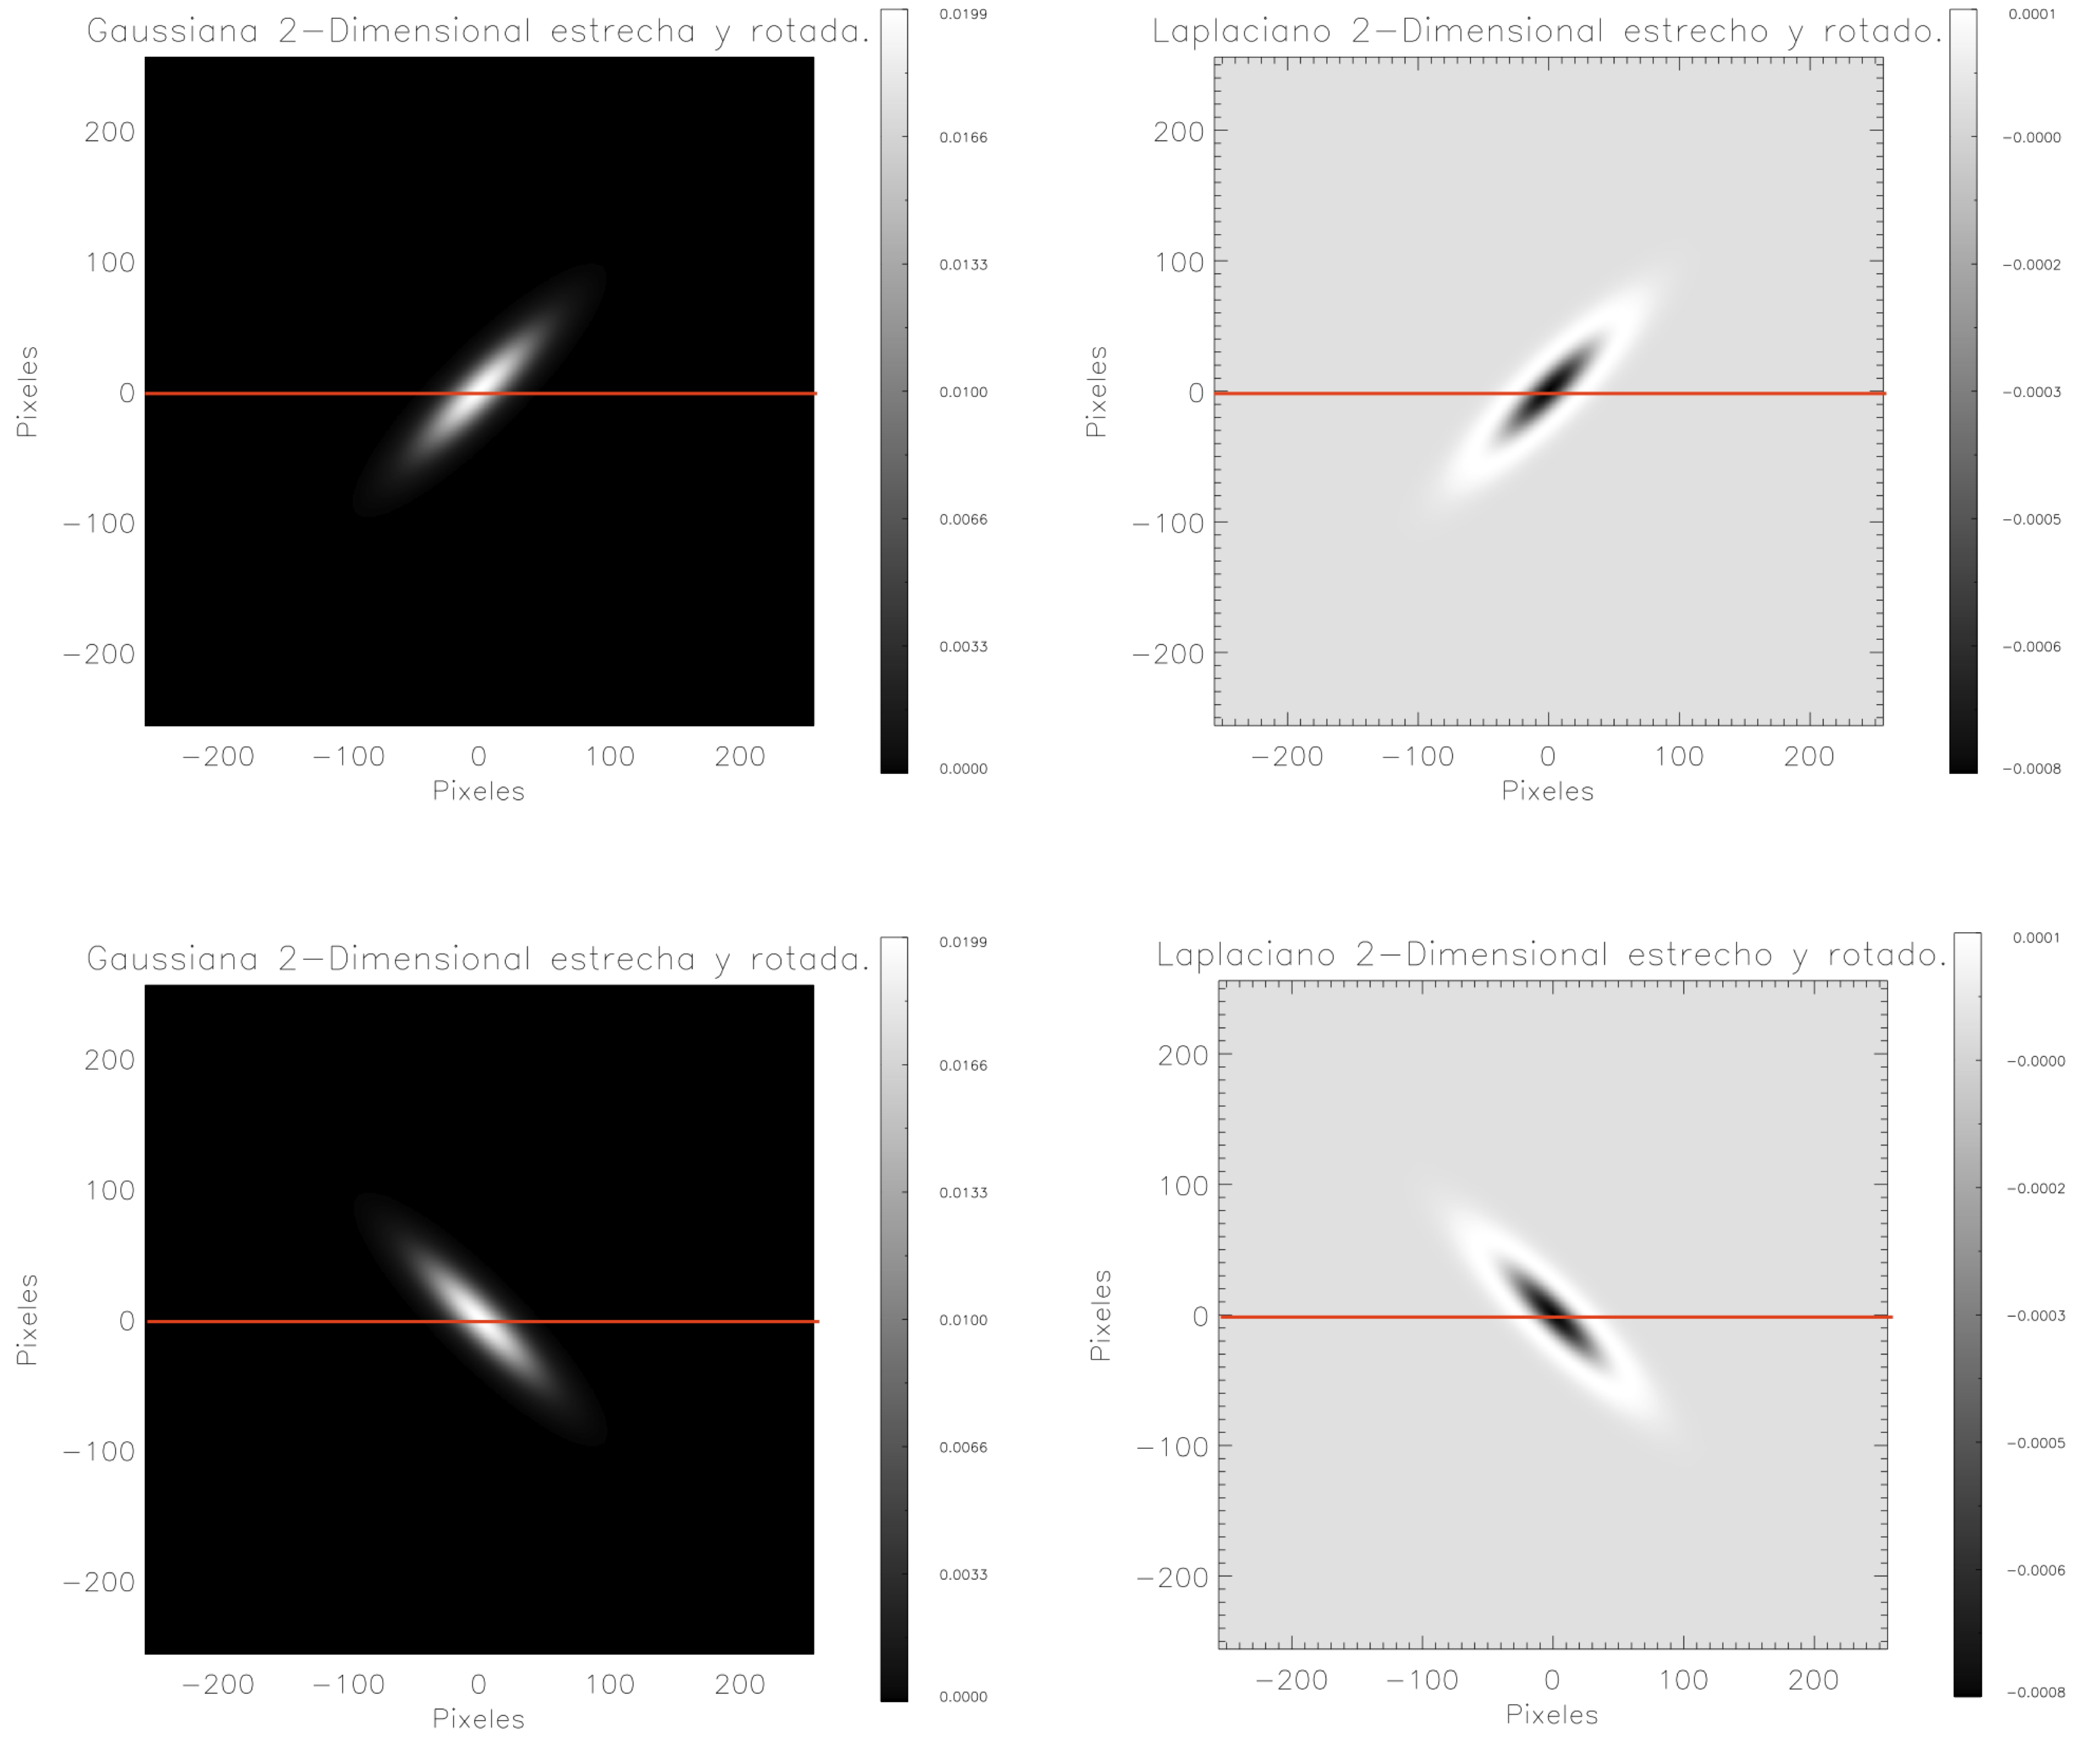
\includegraphics[width=0.7\textwidth]{gausss.png}
\caption{{\it Izquierda:} Se\~nal gaussiana bidimensional que ha sido estirada y luego rotada. {\it Derecha:} Laplaciano te\'orico de cada una de las se\~nales gaussianas a la izquierda. {\it Arriba:} se\~nal gaussiana rotada $45^\circ$. {\it Abajo:} Se\~nal gaussiana rotada $315^\circ$. Las l\'ineas rojas indican el eje de corte escogido para trazar el perfil de cada una de las se\~nales para ser comparados con los algoritmos de c\'alculo num\'erico.}
\label{fig:gausssquezee}
%\end{center}
\end{SCfigure}


\begin{figure}
\begin{center}
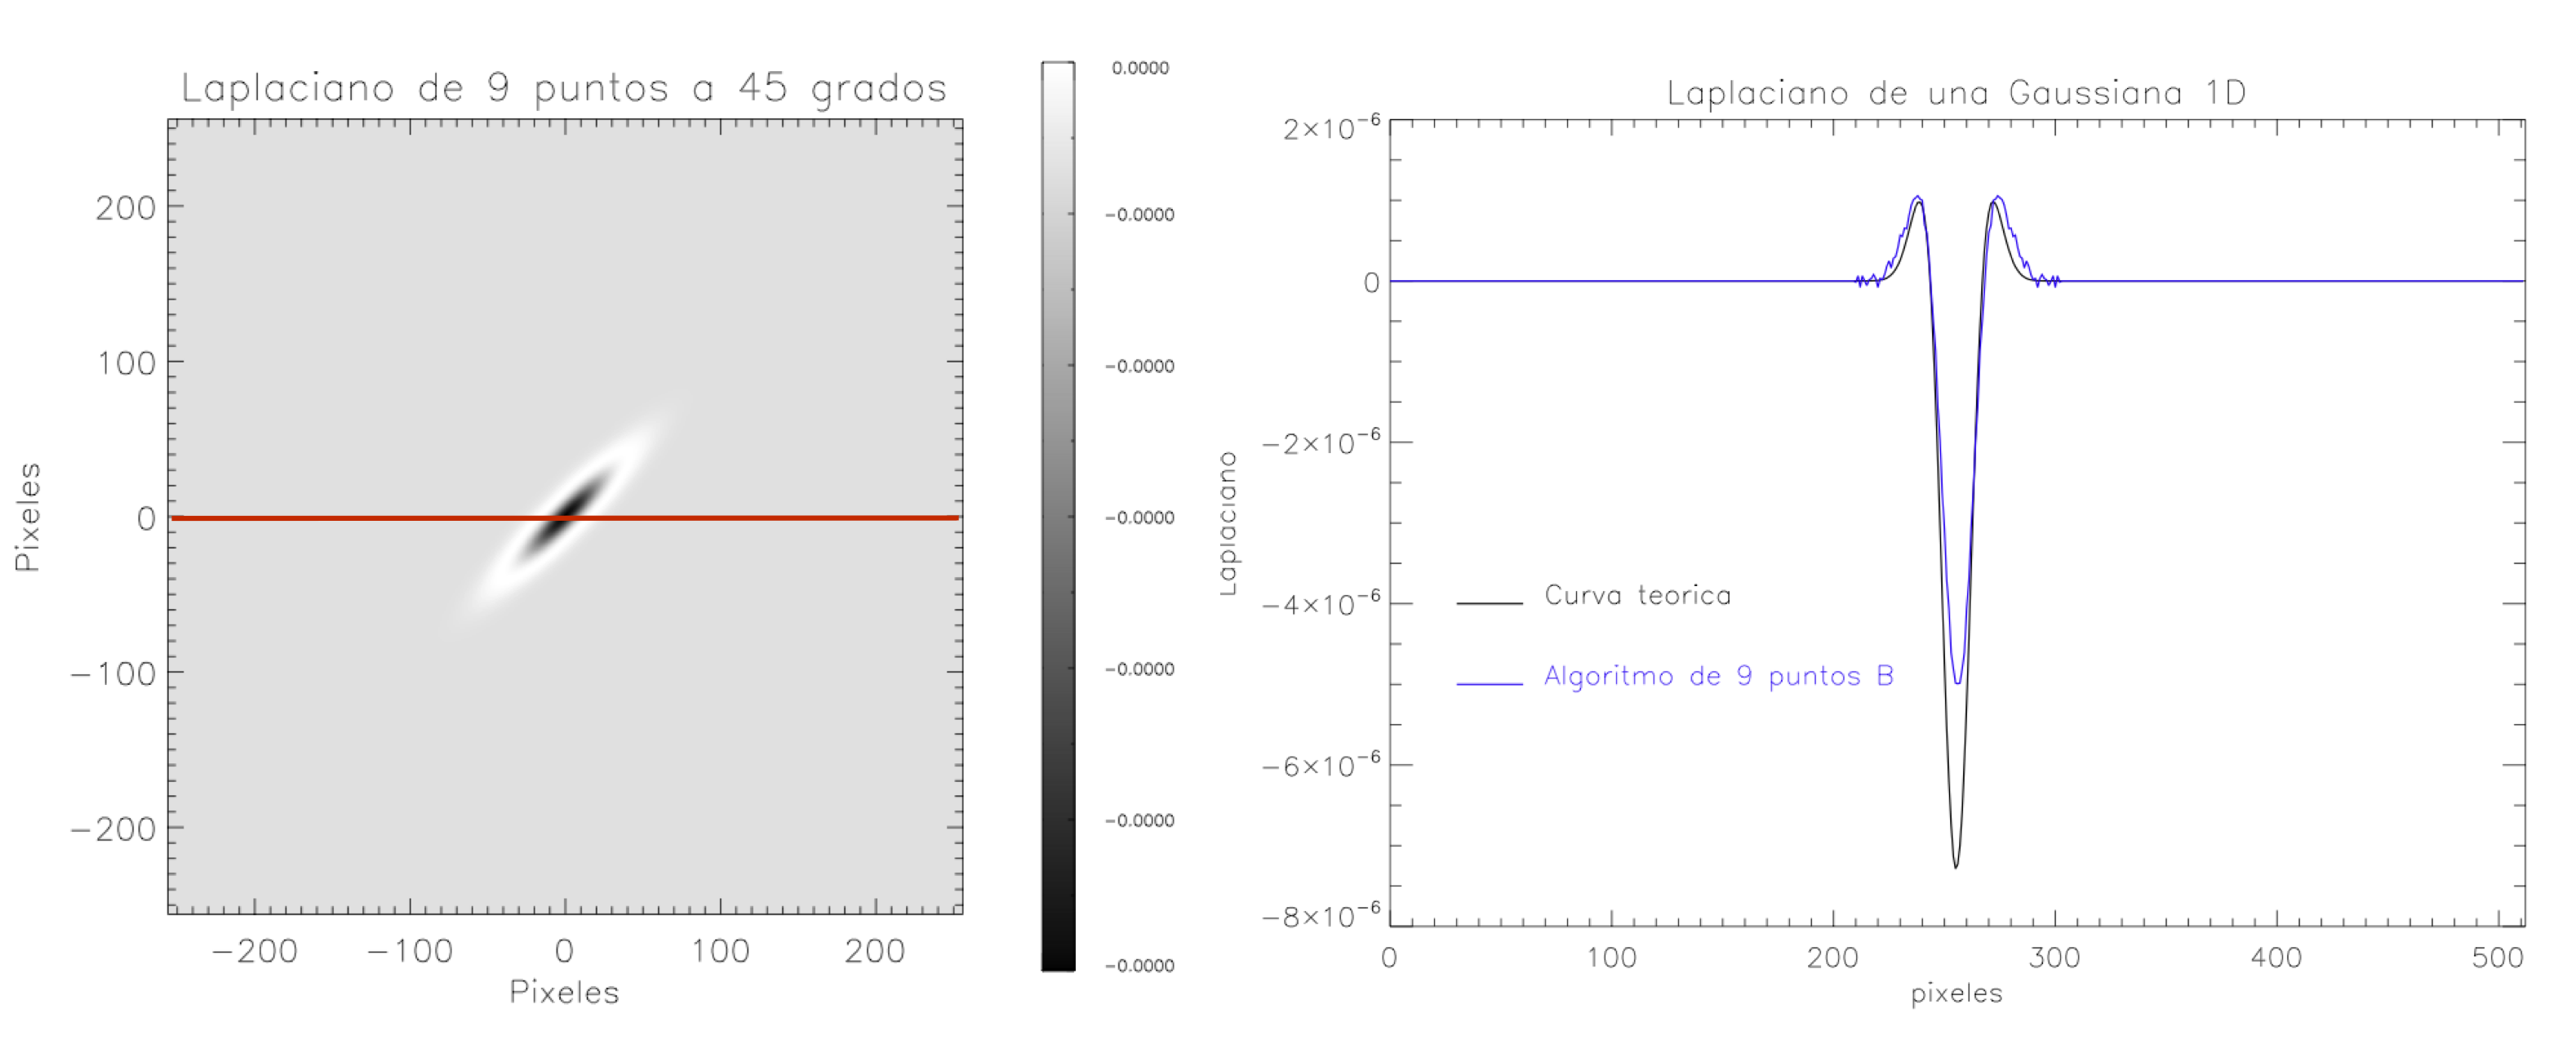
\includegraphics[width=0.95\textwidth]{lap_sq_45.png}
\caption{{\it Derecha}: Laplaciano dos dimensional de una gaussiana achatada y rotada $45^\circ$ calculado con el algoritmo dado por la ecuaci\'on \ref{eq:lapmod} con $\alpha=1.0$, $\beta=1.0$, $\gamma=1.6$. La l\'inea roja indica el lugar por donde se traz\'o el perfil unidimensional que se muestra en la gr\'afica de la {\it izquierda}. El error promedio encontrado entre el ajuste num\'erico y la curva te\'orica es del $5\%$.}
\label{fig:lapjc45}
\end{center}
\end{figure}


\begin{figure}
\begin{center}
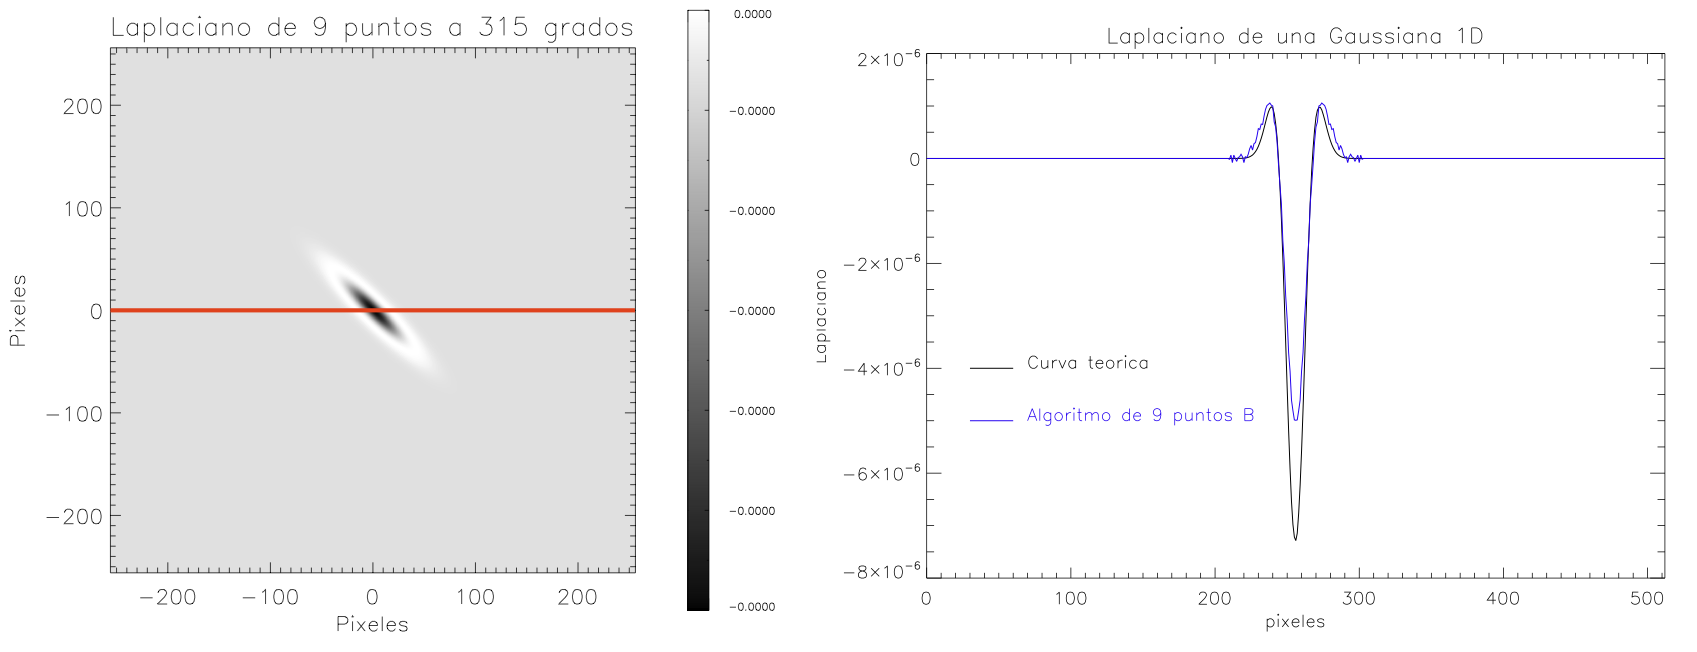
\includegraphics[width=0.95\textwidth]{lap_sq_315.png}
\caption{{\it Derecha}: Laplaciano dos dimensional de una gaussiana achatada y rotada $315^\circ$ calculado con el algoritmo dado por la ecuaci\'on \ref{eq:lapmod} con $\alpha=1.0$, $\beta=1.0$ y $\gamma=-1.6$. La l\'inea roja indica el lugar por donde se traz\'o el perfil unidimensional que se muestra en la gr\'afica de la {\it izquierda}. El error promedio encontrado entre el ajuste num\'erico y la curva te\'orica es del $5\%$.}
\label{fig:lapjc315}
\end{center}
\end{figure}

Ahora bien, con este conjunto de pruebas que se han hecho sobre la forma en la que se debe modificar el algoritmo que calcula el laplaciano de nueve puntos sobre una se\~nal que no es homog\'enea ni isotr\'opica, y al comprobar su correcto funcionamiento, lo que nos ata\~ne ahora es encontrar la forma en la que estos coeficientes $\alpha$, $\beta$ y $\gamma$, que dan peso a los p\'ixeles de la vecindad dependiendo de la geometr\'ia de la se\~nal, deben ser definidos para que este procedimiento de c\'alculo num\'erico pueda ser aplicado correctamente sobre una se\~nal f\'isica real proveniente de alg\'un lugar sobre la superficie solar. En este orden de ideas debemos relacionar el valor de estos tres coeficientes con una proyecci\'on postel que se haga del fotograma tomado del Sol centrado en la regi\'on de inter\'es, la regi\'on activa asociada a la fulguraci\'on que en nuestros casos pudo dar pie a la generaci\'on de un helio-sismo.

\subsection*{Proyecciones heliogr\'afica y postel aplicadas a un fotograma solar}
\addcontentsline{toc}{subsection}{Proyecciones heliogr\'afica y postel aplicadas a un fotograma solar}

La red de telescopios en tierra GONG++ nos ha prove\'ido de fotogramas de muy buena calidad y resoluci\'on desde Julio de 2001. As\'i, se ha convertido en una fuente importante de datos para el desarrollo de an\'alisis basados en las t\'ecnicas propias de la heliosismolog\'ia; nosotros en particular estamos interesados en heliosismolog\'ia local. Para este tipo de an\'alisis es necesario proveerse de unos arreglos de datos en tres dimensiones conocidos en la comunidad de cient\'ificos solares como {\it cubo de datos}. Esto es, dado el deseo de caracterizar temporalmente una regi\'on determinada que se encuentra sobre la superficie solar es necesario hacer un seguimiento de esta al transcurrir el tiempo. De esta manera este conjunto de datos espacio-temporal se puede definir en la pr\'actica mediante el uso de un arreglo (o cubo de datos) de $N_x\times N_y\times N_t$ elementos, en donde $N_x$ y $N_y$ representan el n\'umero de elementos en cada una de las dimensiones espaciales, y $N_t$ es el n\'umero de pasos temporales. Claramente, la calidad del an\'alisis heliosismol\'ogico que se desarrolle va a depender fuertemente de la calidad de la forma en la que se construya dicho cubo de datos, y de aqu\'i la importancia de este procedimiento.\\

En un marco de referencia geoc\'entrico el Sol no es para nada un objeto inmutable y/o en reposo. El Sol tiene un movimiento anual de traslaci\'on a lo largo de la ecl\'iptica, un movimiento de rotaci\'on con respecto a su eje polar y unos movimientos m\'as finos dados por la precesi\'on y nutaci\'on de su eje polar. El conjunto completo de estos movimientos debe ser corregido por un seguimiento excelso de la regi\'on de inter\'es en aras de construir un cubo de datos adecuado. Para esto \cite{lb2000} han propuesto un par de transformaciones, una transformaci\'on heliogr\'afica acompa\~nada de una proyecci\'on {\it Postel}, en el marco de la definici\'on de su m\'etodo propio de {\it holograf\'ia ac\'ustica}.\\

La primera transformaci\'on que se lleva a cabo es una transformaci\'on de coordenadas heliogr\'aficas a coordenadas cartesianas helioc\'entricas. Para esto es necesario conocer la longitud de {\it Carrington}, $L_{ij}(t_k)$, y la latitud heliogr\'afica\footnote{Estas coordenadas son conocidas como las {\it coordenadas de Carrington}. Estas coordenadas son una variaci\'on del sistema coordenado heliogr\'afico que rota a una velocidad angular igual a la tasa de rotaci\'on media del Sol tal y como fue definido originalmente por Carrington (1863). El periodo sideral del sistema de Carrington es de 25.38 d\'ias, lo cual implica un periodo sin\'odico de 27.2753 d\'ias. \cite[]{thompson2005}}, $B_{ij}(t_k)$, para todo elemento con coordenadas $i,j$ en todo $t_k$, en donde $i\in N_x$, $j\in N_y$ y $t_k\in N_t$. Esto es posible, si en particular se conocen las coordenadas de Carrington de un determinado punto sobre el disco solar. Para este fin, cada uno de los observatorios de la red GONG++ registra en los {\it encabezados} de los archivos fits las coordenadas de {\it Carrington} instant\'aneas del punto {\it sub-tierra}, que es aquel punto que se genera en la intersecci\'on de la la superficie solar con la l\'inea recta que une al centro de la tierra con el centro del Sol (instant\'aneos) cada vez que se toma un fotograma. Esto, salvo un peque\~no error por paralaje, coincide con el punto ubicado en el centro del disco solar definido sobre las im\'agenes que se toman. De esta manera, para poder hacer una descripci\'on completa es necesario definir un tiempo de referencia para el punto central: $M_0=M_{00}(t_0)$ dado por $B_0=B_{00}(t_0)$ y $L_0=L_{00}(t_0)$. Adem\'as, se necesita definir un conjunto de im\'agenes ordenadas temporalmente seg\'un el momento en el que fueron tomadas y separadas por el tiempo caracter\'istico dado por la cadencia de los instrumentos que se est\'an usando para la medida (en el caso de GONG la cadencia es de un minuto). As\'i, $t_k=t_0+k\Delta t$ donde $\Delta t$ es la cadencia caracter\'istica de los instrumentos y $k=-N_t/2,...,-1,0,1,...,N_t/2$.\\

\begin{figure}
\centering
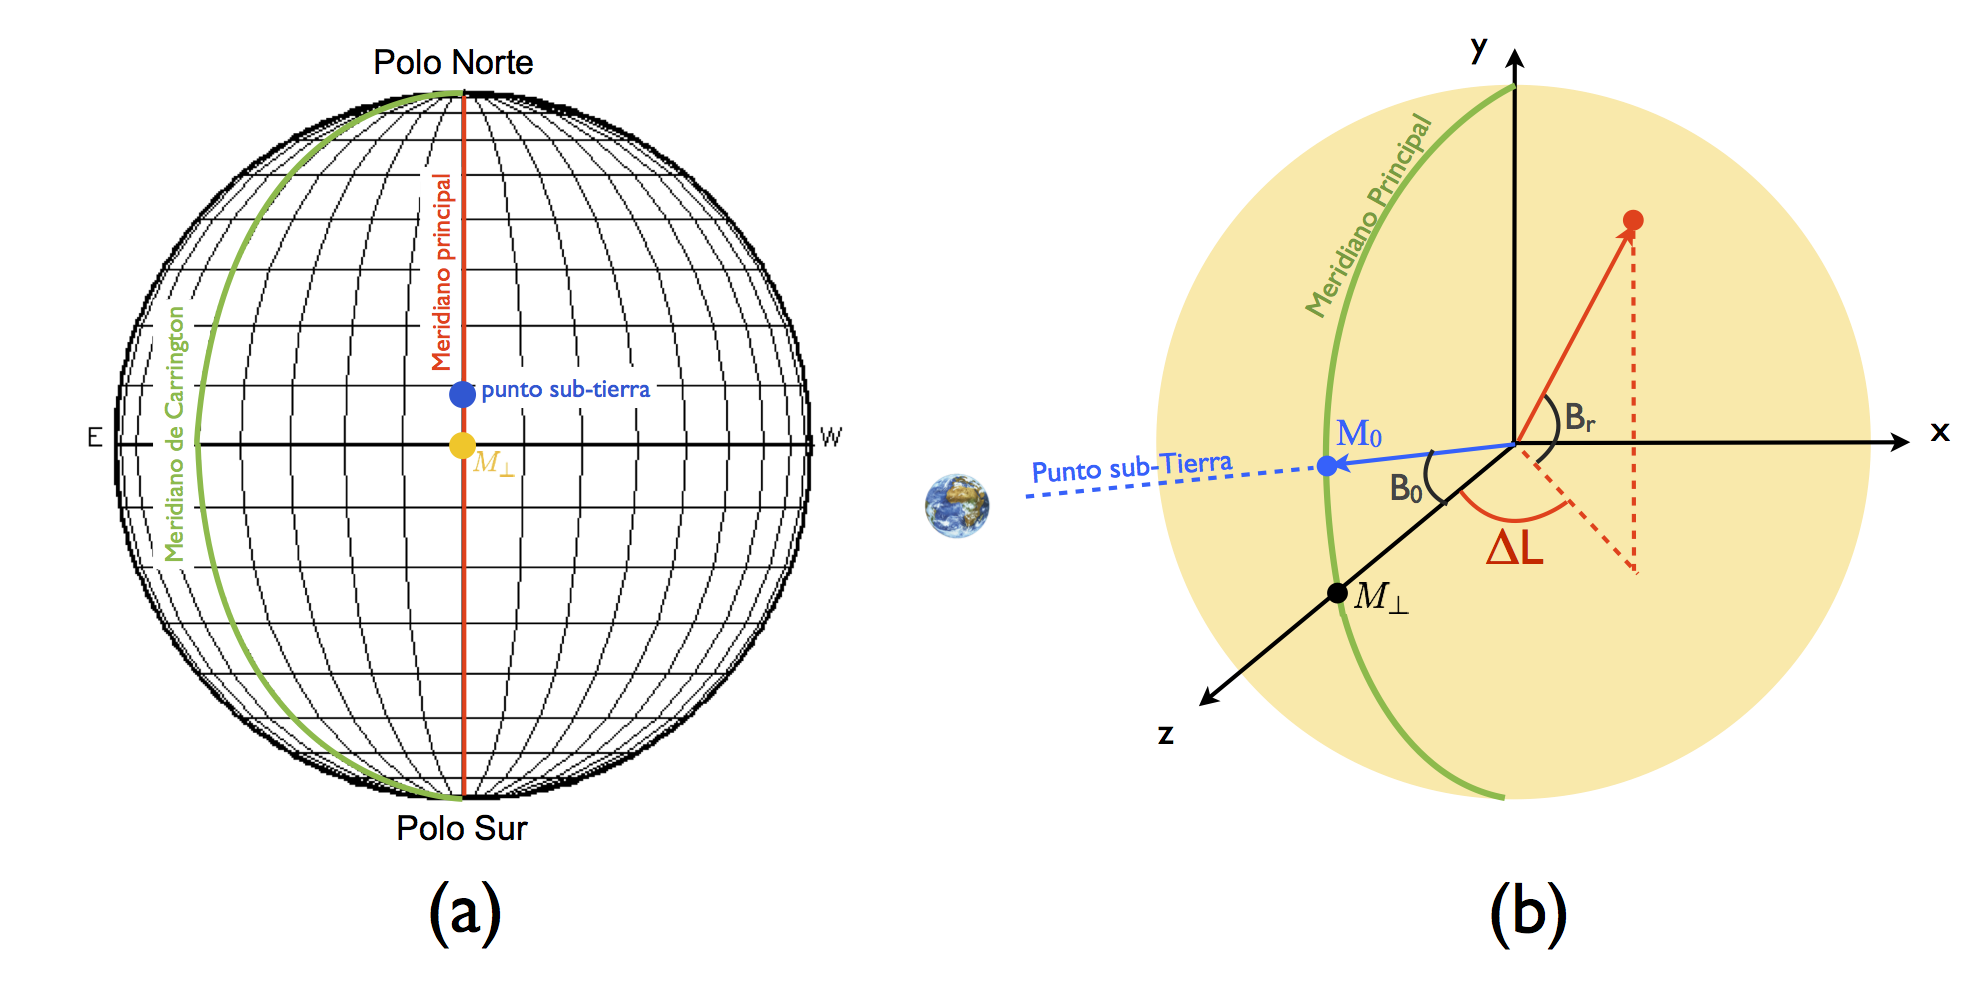
\includegraphics[width=0.65\textwidth]{carrington1.png}
\caption{{\bf (a)}. Representaci\'on gr\'afica del {\it punto sub-tierra} (en azul), el meridiano principal (en rojo), el meridiano de Carrington (en verde) y el punto de intersecci\'on entre el meridiano principal y el c\'irculo m\'aximo perpendicular a \'el en un marco de referencia heliogr\'afico cuya grilla se indica en negro. {\bf (b)} Sistema coordenado cartesiano en tres dimensiones, con origen en el centro del solar, en donde se definen el punto {\it sub-tierra} (punto azul sobre la superficie), el meridiano principal (semic\'irculo verde), y el punto $M_\bot$ en la intersecci\'on entre el meridiano principal y el c\'irculo m\'aximo helioc\'entrico perpendicular al eje $y$. Un punto arbitrario sobre la superficie solar se puede ubicar mediante la asignaci\'on de valores $\Delta L$ y $B_r$.}
\label{fig:carrington}
\end{figure}

Adem\'as, denotamos como $R$ al sistema de coordenadas heliogr\'aficas de {\it Carrington},  sobre \'el $M_0$ es el punto {\it sub-tierra}, $M$ representa al meridiano principal (en ingl\'es {\it prime meridian}), el cual se define como el semic\'irculo m\'aximo que une a los dos polos heliogr\'aficos y que contiene a $M_0$. El punto $M_{\bot}$ se define como la intersecci\'on entre el meridiano principal y el c\'irculo m\'aximo trazado sobre la heliosfera perpendicular a \'el ({\it ecuador solar}), tal como se esquematiza en la figura \ref{fig:carrington}(a).  Podemos introducir un sistema cartesiano de coordenadas con origen en el centro del Sol, cuyo eje $y$ est\'a orientado a lo largo del eje polar, y el eje $z$ est\'a orientado en la direcci\'on radial hacia el punto $M_\bot$.  Una transformaci\'on entre las coordenadas heliogr\'aficas esf\'ericas, por el momento con radio unitario, y las coordenadas cartesianas definidas arriba, viene dada por el siguiente conjunto de ecuaciones:

\begin{align}
\begin{pmatrix}
x\\
y\\
z
\end{pmatrix}
=
\begin{pmatrix}
\cos B_{xy}\sin L_{xy}\\
\sin B_{xy}\\
\cos B_{xy}\cos L_{xy}
\end{pmatrix},
\end{align}

\noindent esto para un determinado tiempo $t_k$. Ahora bien, la necesidad de manipular las im\'agenes del Sol de forma tal que queden perfectamente alineadas una detr\'as de la otra a la hora de construir el cubo de datos nos enfrenta a la necesidad de corregir las im\'agenes por el conjunto completo de movimientos que afectan a la visual del disco solar minuto a minuto en el registro de los fotogramas, adem\'as de hacer una proyecci\'on {\it Postel} correcta sobre la regi\'on de inter\'es. Supongamos que nuestra regi\'on de inter\'es est\'a en una posici\'on arbitraria sobre el disco solar, como se representa mediante el punto rojo en la figura \ref{fig:carrington}(b). A dicho punto le corresponden las coordenadas heliogr\'aficas $L_r$ (longitud de {\it Carrington}) y  $B_r$ (latitud de {\it Carrington}). As\'i, en el sistema coordenado R de la figura \ref{fig:carrington}(b) las coordenadas helioc\'entricas de dicha regi\'on van a estar dadas por

\begin{align}
\begin{pmatrix}
x_r\\
y_r\\
z_r
\end{pmatrix}
=
\begin{pmatrix}
\cos B_r\sin \Delta L\\
\sin B_r\\
\cos B_r\cos \Delta L
\end{pmatrix},
\end{align}

\noindent en donde $\Delta L$ es la diferencia entre las longitudes de {\it Carrington} del punto $r$ y el punto {\it sub-tierra} $M_0$. Ahora bien, un sistema coordenado $R'$ con origen en el centro del Sol y cuyo eje $z'$ se dirige a lo largo del punto {\it sub-tierra} se puede definir a trav\'es de las coordenadas en $R$ mediante una rotaci\'on coordenada sencilla a lo largo del eje $x$, como se esquematiza en la figura \ref{fig:rotacion}. De esta manera, las coordenadas de nuestra regi\'on de inter\'es representadas en el sistema coordenado $R'$ estar\'an dadas por:

\begin{align}
\begin{pmatrix}
x'_r\\
y'_r\\
z'_r
\end{pmatrix}
=
\begin{pmatrix}
1 & 0 & 0 \\
0 & \cos B_0 & -\sin B_0\\
0 & \sin B_0 & \cos B_0 
\end{pmatrix}
\begin{pmatrix}
x_r\\
y_r\\
z_r
\end{pmatrix}.
\end{align}

\begin{wrapfigure}[20]{r}{0.45\textwidth}
\begin{center}
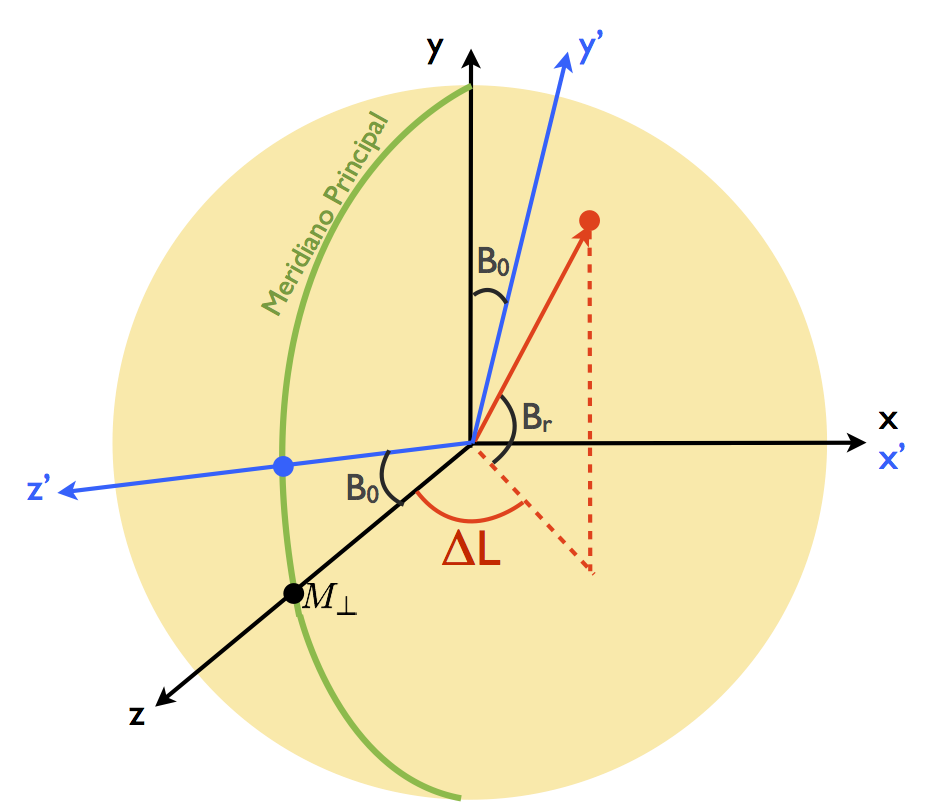
\includegraphics[width=0.42\textwidth]{rotacion.png}
\caption{Definici\'on de un sistema coordenado $R'$, de coordenadas $x',y',z',$ en azul, que est\'a rotado un \'angulo $B_0$ con respecto al eje $x$ del sistema $R$ (en negro).}
\label{fig:rotacion}
\end{center}
\end{wrapfigure}

Como la regi\'on para analizar se puede ubicar en cualquier posici\'on sobre la superficie solar, se sigue inmediatamente que este conjunto de ecuaci\'on es extrapolable a cualquier punto arbitrario, obteniendo de esta manera las ecuaciones expuestas en (\ref{eq:transform}).

\begin{align}\label{eq:coordenadas}
\cos\theta'\sin\varphi'&=\cos B_r\sin\Delta L\\\nonumber
\sin\theta'&=-\cos B_r\sin B_0\cos\Delta L+\sin B_r\cos B_0\\\nonumber
\cos\theta'\cos\varphi'&=\cos B_0\cos B_r\cos \Delta L+\sin B_0\sin B_r.
\end{align}

Con esto se logra alinear apropiadamente todos los fotogramas en la muestra temporal $N_t$ de manera que ya es posible construir el cubo de datos sin problemas, ya que existe un movimiento relativo Sol-observador debido tanto a la rotaci\'on del Sol como al movimiento del observador mismo en su descripci\'on helio\'entrica, de modo tal que para cada instante de tiempo se asume que se conocen $L_0$ y $B_0$ de las efem\'erides f\'isicas del Sol. En seguida, la tarea consiste en llevar a cabo la proyecci\'on {\it Postel} de este \'ultimo sistema coordenado cartesiano $R'$ al plano imagen del fotograma, y para esto hacemos uso de las expresiones mostradas en (\ref{eq:postel}).\\

Siguiendo lo visto en el cap\'itulo anterior, es necesario considerar la posici\'on de la regi\'on de inter\'es sobre el disco solar para poder asignar los pesos correctos al algoritmo de c\'alculo del laplaciano de nueve puntos (\ref{eq:lapmod}) y de esta manera implementar el m\'etodo de limpieza PASCAL sobre las im\'agenes de ciencia sin ning\'un inconveniente. En esta direcci\'on, lo que se hace es definir cuatro par\'ametros $a_{11},a_{12},a_{21},a_{22}$ que forman parte de la matriz $\mathbf{A}$ definida de la siguiente manera:

\begin{align}
\mathbf{A}=
\begin{pmatrix}
a_{11} & a_{12}\\
a_{21} & a_{22}
\end{pmatrix}
=
\begin{pmatrix}
[\sin B_0\sin B_r \cos\Delta L + \cos B_0\cos B_r] & \sin B_r \sin\Delta L\\
-\sin B_0 \sin\Delta L & \cos \Delta L
\end{pmatrix}\frac{1}{z'_r},
\end{align}

\noindent donde 

\begin{align}
\alpha&\equiv a_{11}^2+a_{12}^2\\\nonumber
\beta&\equiv a_{11}^2+a_{12}^2\\\nonumber
\gamma&\equiv 2 (\,a_{11}a_{21}+a_{22}a_{12}).
\end{align}


N\'otese que si la regi\'on de inter\'es se ubica justamente en el centro del disco solar de los fotogramas, es decir, se satisface $\Delta L=0$ y $B_r=B_0$, se cumple que $\alpha=1$, $\beta=1$ y $\gamma=0$; lo que era de esperarse pues en este caso la regi\'on de inter\'es ser\'ia localmente homog\'enea e isotr\'opica y por lo tanto la expresi\'on (\ref{eq:lapmod}) se reduce al algoritmo dado por (\ref{eq:lap5}) con $h=1$.

\section*{Implementaci\'on del m\'etodo PASCAL sobre una muestra de fulguraciones energ\'eticas}
\addcontentsline{toc}{section}{Implementaci\'on del m\'etodo PASCAL sobre una muestra de fulguraciones energ\'eticas}


Como se mencion\'o anteriormente, en la secci\'on de~\nameref{sec:sismicidad}, se han reportado eventos de fulguraciones solares s\'ismicamente activas con una correlaci\'on local fuerte de una emisi\'on grande y repentina en luz blanca. \cite{detal2006} reportaron por primera vez una coincidencia fuerte entre la ubicaci\'on de la fuente s\'ismica, determinada a partir de los mapas de egresi\'on construidos a trav\'es de la t\'ecnica de holograf\'ia ac\'ustica, y tres n\'ucleos compactos y bien definidos de emisi\'on en luz blanca para un evento que tuvo lugar el 9 de Septiembre de 2001 a las 20:40 TU. Esto \'ultimo soporta la hip\'otesis de que el calentamiento repentino de la fotosfera es un proceso que podr\'ia estar ligado a la generaci\'on repentina de una onda mec\'anica transitoria que podr\'ia, a su vez, estar relacionada con la aparici\'on de una fuente s\'ismica. Algunos autores han propuesto diferentes mecanismos posibles que tratan de dar una explicaci\'on plausible de los procesos f\'isicos que podr\'ian estar involucrados detr\'as del calentamiento repentino de la fotosfera. Por ejemplo, \cite{dl2005} y \cite{zharkova2008} argumentan que el calentamiento de la fotosfera podr\'ia ocurrir por la interacci\'on directa de protones energ\'eticos  y/o electrones {\it altamente} energ\'eticos con el ambiente del plasma local. Particularmente  \cite{zharkova2008} le da una prelaci\'on importante a los protones, por encima de los electrones, por su poder alto de penetraci\'on en la materia. Sin embargo, algunos otros trabajos \cite[]{kosovichev2007a} sugieren que los protones acelerados no constituyen una fuente adecuada para dar pie a una respuesta hidrodin\'amica en el plasma de la atm\'osfera solar, y por lo tanto dif\'icilmente podr\'ian estar relacionados con la generaci\'on de la fuente s\'ismica asociada a un {\it sunquake} y, a su vez, con el aumento en la emisi\'on de luz blanca altamente localizada tanto espacial como temporalmente. Aunque en estos trabajos se sugiere el {\it back-warming} como posible mecanismo responsable de la emisi\'on en luz blanca que aqu\'i se menciona, otros trabajos ponen en duda cualquier clase de correlaci\'on entre estos dos fen\'omenos \citep[]{isobe2007,potts2010}.\\

De cualquier manera, y sea como sea que el aumento en la emisi\'on de luz blanca asociada a fulguraciones solares sea producida, trabajos relativamente recientes \citep[]{detal2006,pedram2012} han mostrado una correlaci\'on aparente entre la emisi\'on en luz blanca y algunos heliosismos observados durante la fase impulsiva (definida en la banda de los rayos-X suaves) de aquellas fulguraciones alta o moderadamente energ\'eticas que tuvieron lugar a lo largo del ciclo solar 23. Esto hace que las fulguraciones a las que se les asocia una emisi\'on fuerte en luz blanca se conviertan en buenos candidatos a la hora de buscar eventos fulgurantes s\'ismicamente activos, adem\'as de poder utilizarlos adecuadamente en el estudio y entendimiento de la generaci\'on y din\'amica de los {\it sunquakes}.\\

Por otro lado, en el trabajo extensivo de buscar y caracterizar fulguraciones solares s\'ismicamente activas, todo un conjunto de trabajos que usan las t\'ecnicas de holograf\'ia ac\'ustica y de diagrama de tiempo-distancia \cite[]{besliu2005,detal2006,kz2006c,kosovichev2007a,alvarado2012}, han encontrado un buen n\'umero de eventos en los que las se\~nales s\'ismicas est\'an altamente correlacionadas, tanto temporal como espacialmente, con la aparici\'on de fuentes compactas de emisi\'on en rayos-X duros. Estas observaciones han dado pie a otras tantas explicaciones que tratan de dar cuenta de los mecanismos f\'isicos propios de la fenomenolog\'ia que se esconde detr\'as de la generaci\'on de los heliosismos. Por ejemplo, \cite{zharkova2008} sugiere que la emisi\'on en rayos-X duros de todos estos eventos est\'an relacionados de alguna manera con la precipitaci\'on hacia capas m\'as internas del Sol de part\'iculas altamente energ\'eticas y su posterior dep\'osito de energ\'ia en estas regiones.\\

Dada la importancia de las fulguraciones con una emisi\'on alta en luz blanca, as\'i como en rayos-X duros en el estudio de los {\it sunquakes}, se decidi\'o implementar los c\'odigos de limpieza del m\'etodo PASCAL sobre una muestra de fulguraciones que en lo posible tuvieran estas dos caracter\'isticas, as\'i como la de estar localizadas cerca del centro del disco solar en donde los Dopplergramas ofrecen una confiabilidad mayor. Adem\'as, decidimos centrar nuestra atenci\'on sobre los eventos ocurridos en lo que llevamos del ciclo solar 24, pues es el periodo temporal que en estos momentos nos ofrece el mayor n\'umero de fulguraciones sin explorar. En esta direcci\'on, se empez\'o por hacer un filtrado de la lista completa de fulguraciones observadas por el instrumento espacial RHESSI. Para ello, acudimos a la lista publicada permanentemente en \hyperref[http://hesperia.gsfc.nasa.gov/rhessi2/home/data-access/rhessi-data/flare-list/]{http://hesperia.gsfc.nasa.gov/rhessi2/home/data-access/rhessi-data/flare-list/}, y tomamos aquellas fulguraciones que hayan registrado una emisi\'on discernible por los detectores en energ\'ias por encima de los 50 keV y que hayan tenido lugar en el periodo comprendido entre el 1 de Enero de 2010 y el 30 de Julio de 2012\footnote{El 30 de Julio de 2012 fue el \'ultimo d\'ia en que se revis\'o la lista de fulguraciones de RHESSi en el marco de esta tesis. Claramente como para esta fecha a\'un no estamos en el m\'aximo de actividad solar de este ciclo, se espera que en fechas posteriores se encuentren m\'as fulguraciones con las caracter\'isticas que buscamos.}. De esta manera obtuvimos un total de 51 eventos, de los cuales s\'olo 28 ten\'ian una ubicaci\'on cercana al centro del disco solar adecuadas para desarrollar un an\'alisis heliosismol\'ogico. Es de se\~nalar adem\'as que de estas \'ultimas 28 fulguraciones 4 registraron una emisi\'on discernible por RHESSI en la banda de los 100 keV a los 300 keV. Para escoger  estas 28 fulguraciones se procedi\'o a calcular su distancia al centro del disco solar haciendo uso de las coordenadas helioc\'entricas \cite[]{thompson2005} de la fulguraci\'on dadas por RHESSI. Los 28 eventos que se muestran en el cuadro \ref{tb:fulguraciones} son tales que su distancia al centro del disco solar es menor que 600 segundos de arco.\\

El paso siguiente fue buscar los respectivos fotogramas en intensidad de cada uno de los  eventos de la tabla \ref{tb:fulguraciones}. Esto se hizo a trav\'es del servidor oficial de la red GONG++, \hyperref[http://gong2.nso.edu/archive/patch.pl?menutype=s]{http://gong2.nso.edu/archive/patch.pl?menutype=s}. No todos los eventos fueron observados por los telescopios de la red, algunas veces  por malas condiciones atmosf\'ericas, as\'i como por alg\'un posible problema en la calibraci\'on de los datos. De aqu\'i que solamente los {\bf 10} eventos que se se\~nalan en el cuadro \ref{tb:fulguraciones} son de los que se tienen datos de estos instrumentos. As\'i mismo, se aprovecha el cuadro \ref{tb:fulguraciones} para se\~nalar aquellos eventos para los cuales el {\it Helioseismic and Magnetic Imager} a bordo del {\it Solar Dynamic Observatory}, y del que hablaremos m\'as adelante en detalle, registr\'o datos. 

\begin{table}
\caption{Lista de fulguraciones altamente energ\'eticas registradas por RHESSI en rayos-X duros, con emisiones por encima de los 50 keV, durante el periodo comprendido entre el 1 de Enero de 2010 y el 30 de Julio de 2012. La primera columna numera cronol\'ogicamente los eventos, la segunda columna muestra la fecha en la que ocurrieron; las tercera, cuarta y quinta columnas muestran el comienzo, el pico y el final de la emisi\'on en una banda entre los y los keV para cada uno de los eventos respectivamente. La sexta y la s\'eptima columnas muestran la ubicaci\'on de la fulguraci\'on. La novena columna da el n\'umero de la regi\'on activa, y en las casillas d\'ecima y und\'ecima se\~nalamos si el evento fue registrado por la red GONG y/o por HMI/SDO respectivamente.}
\begin{center}
\begin{tabular}{l r r r r r r r r r r}
\toprule[0.8mm]
\# &    Fecha        & Comienzo &      Pico      &     Final     &   X   &   Y    &   AR   & GONG & HMI/SDO\\
\bottomrule[0.8mm]
1   & 2010-02-08 &  07:31:16   &  07:41:26  & 07:53:32  &  034 & 474 & 1045  & &  \\
2   & 2010-02-12 &  11:21:28   &  11:26:14  & 11:36:24  & -169 & 515 & 1046  & \checkmark  & \checkmark  \\
3   & 2010-10-16 &  19:08:48   &  19:12:18  & 19:34:40  & 394 & -397 & 1112  & \checkmark  & \checkmark  \\
4   & 2011-02-14 &  04:41:12   &  04:44:10  & 05:25:04  & 031 & -223 & 1158  & \checkmark  & \checkmark  \\
5   & 2011-02-15 &  01:43:44   &  01:55:30  & 02:27:32  & 205 & -222 & 1158  & \checkmark  & \checkmark  \\
6* & 2011-03-07 &  19:40:12   &  20:04:54  & 20:07:48  & 624 & 556 & 1164  & \checkmark  & \checkmark  \\
7   & 2011-03-09 &  23:10:28   &  23:22:18  & 23:38:08  & 191 &  272 &  ---  & \checkmark  & \checkmark  \\
8   & 2011-07-30 &  02:05:32   &  02:09:10  & 02:29:24  & -526 & 170 & 1261  & \checkmark  & \checkmark  \\
9   & 2011-08-03 &  04:29:24   &  04:31:58  & 04:43:28  & -155 & 166 &  ---  & \checkmark  & \checkmark  \\
10 & 2011-08-04 &  03:42:28   &  03:46:58  & 03:47:40  &  537 & 201 & ---   & \checkmark  & \checkmark  \\
11*& 2011-09-06 &  22:08:00   &  22:19:46  & 22:25:04  &  284 & 133 & 1283   & \checkmark  & \checkmark  \\
12 & 2011-09-08 &  15:33:00   &  15:43:50  & 16:02:00  &  610 & 147 & 1283  & \checkmark  & \checkmark  \\
13 & 2011-09-26 &  05:05:16   &  05:07:58  & 05:14:40  &  -519 & 116 & 1302  & \checkmark  & \checkmark  \\
14 & 2011-12-25 &  20:24:12   & 20:27:54  & 20:35:52  &  369 & -334 & 1387  & \checkmark  & \checkmark  \\
15 & 2011-12-27 &  04:07:32   & 04:18:38  & 04:38:36  &  -494 & -250 & 1386  & \checkmark  & \checkmark  \\
16*& 2012-03-04 &  11:06:52   & 11:07:30  & 11:10:44  &  617 & -666 & ---  & \checkmark  & \checkmark  \\ 
17 & 2012-03-09 &  04:24:36  & 04:27:54  & 04:37:08  &  0 & 389 & 1429  & \checkmark  & \checkmark  \\
18 & 2012-05-09 &  12:29:48  & 12:30:30  & 12:43:00  &  -488 & 242 & 1476  & \checkmark  & \checkmark  \\
19 & 2012-05-09 &  14:10:04  & 14:10:46  & 14:27:32  &  -353 & 162 & 1476  & \checkmark  & \checkmark  \\
20 & 2012-05-10 &  04:13:08  & 04:17:42  & 04:29:36  &  -364 & 259 & 1476  & \checkmark  & \checkmark  \\
21*& 2012-06-03 &  17:49:24  & 17:54:46  & 18:01:20  &  -570 & 275 & 1493  & \checkmark  & \checkmark  \\
22 & 2012-07-02 &  19:47:04  & 20:05:18  & 20:11:56  &  -16 & -325 & 1514  & \checkmark  & \checkmark  \\
23 & 2012-07-04 &  09:49:04  & 09:54:26  & 10:14:32  &  289 & -343 & 1515  & \checkmark  & \checkmark  \\
24 & 2012-07-04 &  16:33:00  & 16:37:06  & 16:46:48  &  484 & -184 & 1513  & \checkmark  & \checkmark  \\
25 & 2012-07-05 &  03:26:20  & 03:35:50  & 03:55:16  &  417 & -338 & 1515  & \checkmark  & \checkmark  \\
26 & 2012-07-05 &  11:39:52  & 11:44:14  & 11:53:08  &  495 & -332 & 1515  & \checkmark  & \checkmark  \\
27 & 2012-07-06 &  01:27:16  & 01:39:38  & 02:13:04  &  585 & -322 & 1515  & \checkmark  & \checkmark  \\
28 & 2012-07-12 &  16:49:52  & 16:50:54  & 17:28:08  &  14 & -308 & 1520  & \checkmark  & \checkmark  \\
%\cmidrule(l){2-4}
%Juan&40& 60 & 100 \$\\
%\midrule
%Pedro&70& 30 & 100 \$\\
%\cmidrule[0.5mm](l){4-4}
%& & & 200 \$ \\
\bottomrule[0.8mm]
\end{tabular}
\end{center}
\label{tb:fulguraciones}
\end{table}



%%%%%%%%%%%%%%%%%%%%%%%%%%%%%%%%%%%%%%%%%%%

%\begin{wrapfigure}[20]{r}{0.65\textwidth}
%\begin{center}
%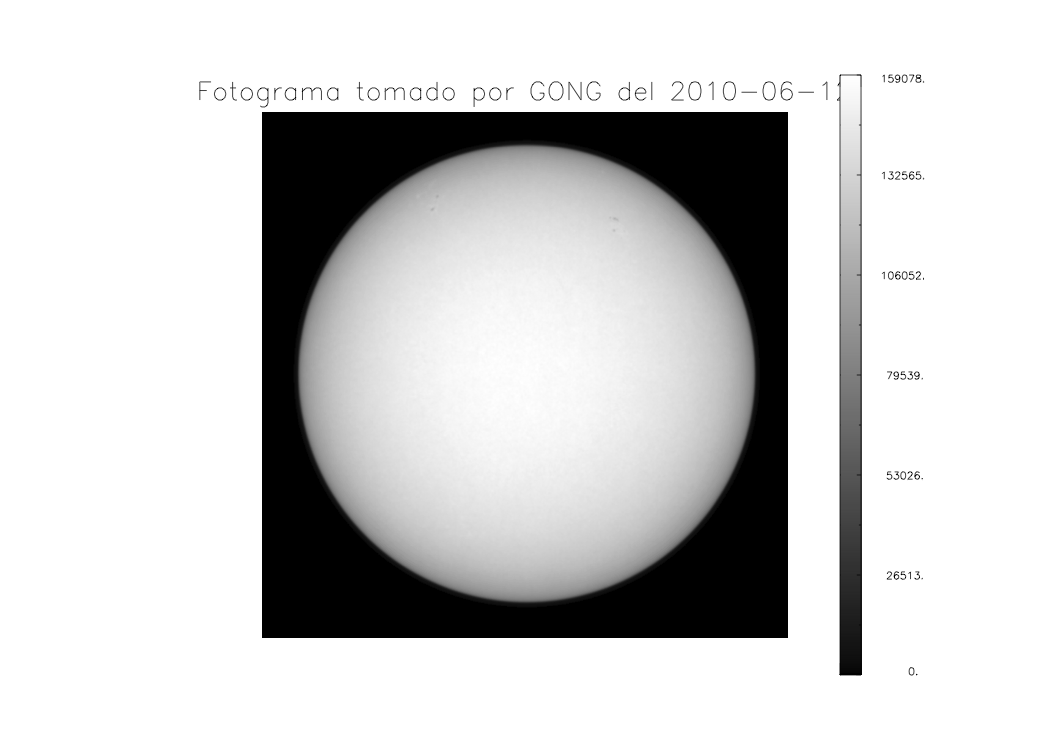
\includegraphics[width=0.65\textwidth]{gong.png}
%\caption{Fotograma en luz blanca del Sol el 12 de Junio de 2012 por el Observatorio Mauna Loa HI USA de la red de telescopios terrestres GONG++.}
%\label{fig:gong}
%\end{center}
%\end{wrapfigure}


%Hablar de que todos los trabajos han considerado m�todos de 5 puntos, y que nosotros lo comparamos con el de 9 y describir lo que encontramos... depu�s hablar de Sergey y sus im�genes mostrar unas de nuestras im�genes si las hay.







